\documentclass[12pt]{article}
\usepackage{amsmath,amssymb}
\usepackage[margin=2cm]{geometry}
\usepackage{float}
\usepackage{graphicx}
\usepackage[semicolon]{natbib}
\usepackage[multiple,bottom]{footmisc}
\usepackage[sc]{caption}
\usepackage{ctable}
\usepackage[para,online,flushleft]{threeparttable}

\linespread{1.1}

% Preferences for equation numbers
\numberwithin{equation}{section}

\title{A Modified Taylor rule to face the Zero Lower Bound}
\author{Damian Romero}
\date{This version: January 5, 2017}

\begin{document}
	
\maketitle

\begin{abstract}
	\noindent In this paper I characterize the dynamics of an stylized version of the New Keynesian model when the economy is subject to demand shocks. First, I compare the evolution of the economy when the zero lower bound is an occasionally binding constraint with the case in which it is not taken into account, to state the main differences of both economies. I find that the constraint significantly reduces the capacity of the central bank to face the shock. Studying a modified Taylor rule, in which past inflation or past output are used to determine current policy, I find that the impact of the shock is reduced in at least 30\%, even when the weight of past macroeconomic variables in the Taylor rule is modest. This result is independent of the variable used by the central bank. The modified policy helps the economy to recover more quickly, avoiding extreme welfare losses. Finally, with the alternative rule, the nominal interest rate spends less than 0.5\% of the time on the zero lower bound, in comparison with a 2\% in the case of a traditional rule.
\end{abstract}	
	
\section{Introduction}\label{sec:introduction}

From the recent financial crisis onwards, central banks in different countries have fought the consequences of fundamental shocks that have had long-term consequences for macroeconomic outcomes. Once the crisis started, monetary authorities have used their policy instruments to face the crisis, which has produced that interest rates plummet up to the point were they attain the so called zero lower bound. Also, central banks around the world have implemented alternative monetary policies to fight the crisis, like quantitative easing policies and forward guidance.\footnote{For an introduction, see \cite{BorioEtAl2016}. For a review about quantitative easing programs, see \cite{ChenEtAl2012} and \cite{JoyceEtAl2012}.} Given this scenario, analyzing the consequences of these kinds of policies had become one of the main tasks for monetary economists, both from a policy and from an academic perspective.\footnote{Some of the first papers to study the properties of these kinds of models are \cite{BenhabibEtAl2001,BenhabibEtAl2001a,BenhabibEtAl2002}, \cite{EggertssonEtAl2003} and \cite{AdamEtAl2007}, when the crisis has not even started. After this, a large body of literature have studied, both theoretically and quantitatively, monetary models subject to the zero lower bound. See for example \cite{Fernandez-VillaverdeEtAl2015} and \cite{AruobaEtAl2016} and the references therein.}

In this paper, I study a simple version of the New Keynesian model when the economy is subject to demand shocks. In order to model those shocks, I introduce an stochastic process for the discount factor of the representative household, so when the discount factor increases (a negative demand shock), this diminishes current consumption, having effects over output, labor demanded by firms and prices. To fully understand the mechanics of the model, I first compare the impulse-response functions of the economy when is subject to the zero lower bound, against the case when this is not considered in the model. As has been illustrated by the literature, the lack of capacity of the monetary authority to reach negative values for the interest rate, makes that the economy suffers a more pronounced crisis. In my calibration, this is reflected with a decrease in output of 1.5\% below its deterministic steady-state level. Also, the central bank keeps interest rates at the zero bound for too long, which reinforces the effect of the shock, keeping the economy in a liquidity trap that sustain the crisis \citep{Werning2012}. Because of the forward-looking nature of the macroeconomic modeling, I also study the effect over expectations of the shock, finding that when the zero bound is present in the model, it has no effect on expectations four or eight periods ahead related to the case when the constraint is not considered. This is, including the bound does not affect expectations relative to the baseline case without the restriction. This result is important because sets a benchmark for alternative policies that could be considered to fight the crisis in terms of how they modify private expectations, affecting the decision making process of the private sector.

The main contribution of the paper comes in the second part, where I study a simple departure from the standard Taylor rule that I call pseudo forward guidance or modified Taylor rule. The objective of forward guidance is to set expectations of future policy (or future policy shocks) in order to affect current macroeconomic variables. Because of rational expectations and the recursive nature of the model, this is analogous to consider a Taylor rule that includes past macroeconomic variables to make a decision of current policy. In this regard, I explore the consequences of using, besides current output and inflation, past values of these variables in the determination of current nominal interest rate. Presenting different specifications of the rule and changing the sensitivity of the central bank to these past variables, I study how the economy reacts in these specifications compared to the standard model (subject to the zero lower bound and using a standard Taylor rule). My main results can be summarized as follows. Using past inflation or past output to determine policy generates similar dynamics; the key element is how sensitive is the rule to the selected variable. I find that the impact of the crisis is severely reduced around a third for inflation and output, and more than a hundred percent for real marginal costs. In the case of interest rate, the central bank reaches the zero bound for only one period, avoiding a liquidity trap. In terms of expectations, the decrease of those is reduced around 100\% for output and inflation, both at four and eight quarters horizon. With this, I find that a simple modification not only diminishes the real impact of the crisis, but also reduces the possibility of getting unanchored expectations.\footnote{For a more detailed analysis of forward guidance policies and their impact on expectations, see \cite{CampbellEtAl2012}, \cite{AndradeEtAl2015}, \cite{BachmannEtAl2015} and \cite{AngeletosEtAl2016}.} As mentioned before, all these gains depends on the degree of reaction of monetary policy to past outcomes, but even in intermediate cases, like a parameter of 0.5 in the modified Taylor rule, produces significant gains. Although simplistic, this representation of the economy shows that a basic modification of the standard policy rule used by central banks could produce significant gains by reducing the impact of shocks in the business cycle, without the need of changing policy targets \citep{CoibionEtAl2012} or using wasteful policies \citep{CorreiaEtAl2013}.

The rest of the paper is organized as follows. The next section describes the environment of the economy, characterizing the equilibrium, calibration, solution method and the pseudo forward guidance (modified monetary policy). In section \ref{sec:results}, I present the results of the analysis, first comparing the model with and without the zero lower bound, to then study the impact of the modified policy rule. Section \ref{sec:conclusions} concludes.

\section{Environment}\label{sec:model}

This section summarizes the optimality conditions that characterize the equilibrium of the New Keynesian model, the calibration used trough the exercises, solution method and some modifications of the baseline model to study alternative monetary policies. 

The economy is inhabited by a representative household that derives utility from consumption and (des-utility from) labor. The household consumes a basket of differentiated goods--which are imperfect substitutes among them--with a constant elasticity of substitution between varieties. There is a continuum of firms in the economy that compete imperfectly, operating with linear technologies. I assume that there are no technology or supply shocks in the economy. This is done for simplicity in order to study the properties of the model when the zero lower bound is attained.\footnote{As \cite{Fernandez-VillaverdeEtAl2015} mentions, a demand shock in the form of a shock to household preferences is the most effective way to attain the zero lower bound. Given their analysis, I use just this shock to characterize the economy.} To characterize the price-adjustment process, I consider a simplified version of the model in the line of \cite{Rotemberg1982}, which proposes that the cost of adjusting those prices corresponds to a fraction of total output. This allows to simplify the problem by eliminating one extra state variable in comparison with a model characterized by Calvo prices.\footnote{Those models include price dispersion among firms, which is a function of relative price of every individual firm with the aggregate price level. Typically, this variable evolves as weighted sum between desired inflation and the product between current inflation and past price dispersion, which makes this variable an additional state of the problem.} Finally, there is a central bank that adjust the nominal interest rate in the economy following a Taylor rule that, in principle, depends only on deviations of current levels of inflation and output with respect to their long-run levels. These long-run levels are targeted moments of the authority. 
%Note that this version of the model, the only driving force corresponds to a preference shock, which distorts the level of the discount factor of the representative household every period. 

\subsection{Equilibrium}\label{sec:model_equilibrium}

In Appendix \ref{app:derivation}, I formally derive the model used in this paper. Here I summarize the optimality conditions of the New Keynesian model with constant technology, preferences shocks and Rotemberg prices in the following set of equations

\begin{align}
	\frac{W_t}{P_t}&=C_t^{\sigma}N_t^{\varphi}\label{eq:m_intra}\\
	1&=R_t\mathbb{E}_t\left\{\beta_{t+1}\left(\frac{C_t}{C_{t+1}}\right)^{\sigma}\frac{1}{\Pi_{t+1}}\right\}\label{eq:m_euler}\\
	(1-\varepsilon)+\varepsilon RMC_t-\zeta(\Pi_t-1)\Pi_t&=-\mathbb{E}_t\left\{\beta_{t+1}\left(\frac{C_t}{C_{t+1}}\right)^{\sigma}\zeta(\Pi_{t+1}-1)\Pi_{t+1}\frac{Y_{t+1}}{Y_t}\right\}\label{eq:m_pricing}\\
	RMC_t&=\frac{W_t}{P_t}\label{eq:m_rmc}\\
	R_t&=\max\left\{\overline R\left(\frac{\Pi_t}{\overline\Pi}\right)^{\phi_{\pi}}\left(\frac{Y_t}{\overline{Y}}\right)^{\phi_{y}},1\right\}\label{eq:m_taylor}\\
	Y_t&=N_t\label{eq:m_product}\\
	Y_t&=\left[\frac{1}{1-(\zeta/2)(\Pi_t-1)^2}\right]C_t\label{eq:m_aggregate}\\
	\log \beta_t&=(1-\rho_{\beta})\log\overline\beta+\rho_{\beta}\log \beta_{t-1}+\sigma_{\beta}\eta_t\label{eq:m_ar1_b}
\end{align}

where \eqref{eq:m_intra} is the intratemporal equilibrium condition of the household, with $W_t$ as the level of nominal wage and $P_t$ as the level of prices in current period; \eqref{eq:m_euler} is the Euler equation that links current consumption with future one, where $\Pi_t\equiv P_t/P_{t-1}$ is defined as gross inflation and $\mathbb{E}_t(\cdot)$ is the conditional expectation operator in period $t$; \eqref{eq:m_pricing} is the New Keynesian Phillips curve, where $\varepsilon$ is the elasticity of substitution between varieties for the demand of households; \eqref{eq:m_rmc} defines the real marginal cost of firms;\footnote{In this version of the model, real marginal cost equal real wage. In general, when technology is not constant these two variables differ. I keep the difference just as a matter of comparison with the rest of the literature.} \eqref{eq:m_taylor} is the Taylor rule that characterizes the way monetary authority sets interest rate, which takes into account the zero lower bound by including the maximum operator between the Taylor rule and a level of gross interest rate equal to one; \eqref{eq:m_product} is the aggregate production function; \eqref{eq:m_aggregate} is the aggregation condition which states that aggregate output must be equal to consumption and the cost of changing prices, where $\zeta$ is the parameter that controls that cost; and \eqref{eq:m_ar1_b} is the law of movement for the discount factor, where $\eta_t\sim N(0,1)$. It is important to note that the Taylor rule used here considers the deviation of current level of activity with respect to its long-run value as the relevant activity measure instead of the output-gap \citep{Gali2015}.

As \cite{BenhabibEtAl2001a} and others have mentioned, the New Keynesian model has a continuum of steady states. In particular, the literature has considered a steady state characterized by a zero inflation rate and a positive interest rate level; a deflationary steady state, with zero interest rate; and a continuum of equilibria in between. In this paper, I focus the analysis on a steady state with both positive inflation and positive interest rate. An interesting extension would be to consider the other extreme case of zero net interest rate.

\subsection{Calibration}

To calibrate the model, I follow the numbers proposed by \cite{Fernandez-VillaverdeEtAl2015}. In Table \ref{tab:calibration}, I summarize the values used in the paper. For the long-run level of the discount factor, I set a value of $\overline{\beta}=0.994$, to match an annual real interest rate of 2.5 annual percent. For the elasticity of substitution, I use a value of $\sigma=2$, following \cite{Gali2015}, which is a standard value in the literature. The Frisch elasticity is set to one, in line with numbers reported in the literature. The elasticity of substitution between varieties is $\varepsilon=6$, which delivers an average mark-up of 20 percent. To calibrate the cost of adjusting prices, I follow the equivalence presented in \cite{AscariEtAl2012}, which states that in a zero steady state inflation, fixing $\zeta=\frac{(\varepsilon-1)\theta}{(1-\theta)(1-\overline{\beta}\theta)}$ generates the same first-order dynamics between a model with Calvo prices and a model with Rotemberg prices, where $\theta$ is the frequency of price adjustment on the Calvo pricing model. Therefore, using a value $\theta=3/4$, which implies a mean duration of prices of four quarters, we set a cost of price adjustment which is roughly $\zeta=59$.\footnote{Note that the equivalence between both models requieres the use of the discount factor of households, which in this case varies over time. I use the long-run value to fix this cost of adjustment.} For the Taylor rule I set $\phi_{\pi}=1.5$ and $\phi_{y}=0.25$, which are the sensitivity of the monetary authority to inflation and output deviations, respectively. The long-run levels of inflation, output and interest rate are $\overline\Pi=1.005$, $\overline Y=0.9416$, and $\overline R=1.011$, respectively, where just the former is exogenously imposed. Finally, the persistence of preferences is $\rho_b=0.8$ and the volatility of the demand shock is $\sigma_b=0.0025$, implying a half-life of about three quarters and an unconditional standard deviation of 0.42 percent. 
%These parameters makes that the model stays around a 13\% of the time at the zero lower bound in the long-run distribution.\footnote{Between July 1954 and November 2016, the Fed fund rate has stayed in a value below 0.5\%--which is the technical zero lower bound--12.95 and 12.80\% of the time, in monthly and quarterly frequency respectively, which is consistent with our calibration.}

% Table generated by Excel2LaTeX from sheet 'Calibration'
\begin{table}[H]
  \centering
  \caption{Calibration}
    \begin{tabular}{lcc}
    \toprule
    Parameter & Symbol & Value \\
    \midrule
    Steady-state discount factor & $\overline{\beta}$ & 0.994 \\
    Elasticity of substitution & $1/\sigma$ & 1/2 \\
    Frisch elasticity & $1/\varphi$ & 1 \\
    Elasticity of substitution between goods & $\varepsilon$ & 6 \\
    Frequency of price adjustment in Calvo & $\theta$ & 0.75 \\
    Rotemberg adjustment cost & $\zeta=\frac{(\varepsilon-1)\theta}{(1-\theta)(1-\overline{\beta}\theta)}$ & 58.9391 \\
    Monetary policy response to inflation & $\phi_{\pi}$ & 1.5 \\
    Monetary policy response to activity & $\phi_y$ & 0.25 \\
    Steady-state inflation  & $\overline{\Pi}$ & 1.005 \\
    Steady-state output & $\overline{Y}$ & 0.9416 \\
    Steady-state interest rate & $\overline{R}=\frac{\overline{\Pi}}{\overline{\beta}}$ & 1.0111 \\
%    TFP persistence & $\rho_a$ & 0.7 \\
%    TFP volatility & $\sigma_a$ & 0.007 \\
    Discount factor persistence & $\rho_b$ & 0.8 \\
    Discount factor volatility & $\sigma_b$ & 0.0025 \\    
    \bottomrule
    \end{tabular}%
  \label{tab:calibration}%
\end{table}%

\subsection{Solution method}

I solve the model using a projection method with a quasi Newton updating scheme. For this, I approximate policy functions for consumption and inflation to then compute the rest of variables in the model. Given those, I use the Euler equation and the New Keynesian Phillips curve (equations \ref{eq:m_euler} and \ref{eq:m_pricing}) to minimize residuals. My convergence criterion is 1e-8.

Given that we are considering the zero lower bound, which is an occasionally binding constraint, I use a piecewise polynomial spline of order one to capture properly the kink generated by the Taylor rule. Because we are interested in the possibility of large demand shocks, we define the state space to cover a total of ten standard deviations (five below the steady-state and five above). Exploring the approximation degree of the solution method, I find that a grid of 20 points for the discount factor, which is the unique state variable of the model, solves the economy accurately enough. To compute expectations, I use a quadrature procedure for Gaussian processes, considering 30 nodes. To check the accuracy of the solution, I use the parameters that solve the model and a larger grid of 100 points to obtain two measures of error in the solution method. First, I obtain the residuals derived from the Euler equation and the New Keynesian Phillips curve. Second, I obtain the error in terms of consumption by computing the relative approximation error $\delta_t$ as follows

\begin{align*}
	[C_t(1-\delta_t)]^{-\sigma}&=R_t\mathbb{E}_t\left\{\beta_{t+1}\left(\frac{1}{C_{t+1}}\right)^{\sigma}\frac{1}{\Pi_{t+1}}\right\}\\
	\delta_t&=1-\frac{\left[R_t\mathbb{E}_t\left\{\beta_{t+1}\left(\frac{1}{C_{t+1}}\right)^{\sigma}\frac{1}{\Pi_{t+1}}\right\}\right]^{-1/\sigma}}{C_t}.
\end{align*}

This last measure gives the error of approximation of the method in terms of consumption units. For example, a value of 0.01 means that the household is making a mistake equivalent to \$1 for every \$100 consumed when choosing consumption in period $t$. For both measures, I present the average error and the maximum absolute error. In Table \ref{tab:app_error} of Appendix \ref{app:accuracy}, I show the results of the accuracy test for selected values of the expanded Taylor rule (see below). The main result is that errors are larger when we consider the modified policy, but those errors are at most 1.6\% on average and 0.79\% as maximum absolute value (when considering past output in the rule). These values are small enough, so I feel comfortable with the degree of accuracy of the numerical approximation.

In order to find the solution, I use as an initial guess the policy function obtained from a first-order approximation around the steady state using \cite{Sims2002} method. With these policies, I find the nonlinear policies that characterize the economy without taking into account the zero bound. Finally, I use these latter policies as initial guess to find the policies when the economy is subject to the zero lower bound.

\subsection{The model under alternative monetary policies: pseudo forward guidance}

The literature has modeled forward guidance by considering deterministic paths of the monetary policy instrument (or the monetary policy shock) for a given number of periods. Examples of this approach are \cite{DelNegroEtAl2015}, \cite{KaplanEtAl2016} and \cite{McKayEtAl2016}. One exception is \cite{KeenEtAl2016}, which solves a version of the New Keynesian model considering different configurations for the monetary policy shock in terms of the amount of periods that the shock is leaded.

Here I follow an alternative way of dealing with forward guidance, which I call pseudo forward guidance or modified Taylor rule. Given the recursivity of the problem and the Markovian nature of the shock, all relevant information for the decision making process of agents in the model is summarized in the state variable that comes from the period before. With this, by including a past variable in the policy rule, the monetary authority is also concerned about the development of macroeconomic variables across time. Because of rational expectations, private agents internalize this and are aware that the authority not only reacts to current inflation and output, but to previous levels of those variables. Given this, I propose two variations of the Taylor rule given in equation \eqref{eq:m_taylor}

\begin{align}
	R_t&=\max\left\{\overline R\left(\frac{\Pi_t}{\overline\Pi}\right)^{\phi_{\pi}}\left(\frac{Y_t}{\overline{Y}}\right)^{\phi_{y}}\left(\frac{Y_{t-1}}{\overline{Y}}\right)^{\phi_{FG}},1\right\}\label{eq:m_taylor_fg1}\\
	R_t&=\max\left\{\overline R\left(\frac{\Pi_t}{\overline\Pi}\right)^{\phi_{\pi}}\left(\frac{Y_t}{\overline{Y}}\right)^{\phi_{y}}\left(\frac{\Pi_{t-1}}{\overline\Pi}\right)^{\phi_{FG}},1\right\}\label{eq:m_taylor_fg2}
\end{align}

In \eqref{eq:m_taylor_fg1}, I add deviations of past level of output with respect to the steady state level, while in \eqref{eq:m_taylor_fg2} I use past level of inflation. In this case we include a new parameter, $\phi_{FG}$, that controls the relevance that past outcomes have for the authority. Latter on, I study the different implications of solving the model with both specifications and different degrees of relevance of the forward guidance policy. Note that in equations \eqref{eq:m_taylor_fg1}-\eqref{eq:m_taylor_fg2} the model is written with respect to variables in the past. However, this is the same as write the model in a forward looking way, hence, these modifications can be considered as a pseudo forward guidance policy.

\section{Results}\label{sec:results}

In this section I analyze the results derived from the model. First, I compare the response of the economy with and without the zero lower bound constraint to a negative demand shock. After this, I study in which way the response of the main variables react when the pseudo forward guidance policy comes into play, in comparison with the case when policy only reacts to current macroeconomic variables. In each case, I analyze how current variables react and how expectations change with the shock using different policies.

\subsection{Zero lower bound vs no zero lower bound}

To study how different are the responses of the economy with and without the zero lower bound constraint, I analyze the impact that a large negative demand shock has on the model. This shock corresponds to a one-time increase in the discount factor, which increases the value of future utility stream, inducing a desire in increase savings and reducing current consumption. For all the exercises that comprehend impulse-response functions, I use the same simulated process for the discount factor, where the perturbation is a shock of five times the standard deviation in the discount factor.

In Figure \ref{fig:irfLevel_pref}, I show the responses of inflation, output, real marginal cost and interest rate to the negative demand shock, which are the variables that summarize the model. All responses are in percentage deviations with respect to the deterministic steady state, except interest rate which is in gross terms. In this case, we note that the shock generates a decrease in the level of all variables, regardless of considering the zero lower bound or not. The increase in savings--produced by the larger valuation of future utility--implies a direct decrease in consumption, hence on output and hours worked. With this, the interest rate level decreases, strongly in the case of the model without the zero lower bound to a -0.5\%, and up to 0\% in the case of the constrained model. With the decrease in demand we also observe a decrease in the level of prices and (des)inflation, which is traduced to a reduction in the real marginal cost, because of the reduction in the amount of labor demanded by firms. Note that in the case of the model without the zero lower bound mechanism, the response of the interest rate is aggressive enough to minimize the fluctuation in the rest of macroeconomic variables. In particular, the negative level of the interest rate allows inflation and output to be reduced only about 1 and 0.8\% respectively. In the case when the zero lower bound constraint is included, the monetary authority does not have as much room to act in response to the demand shock. In particular, the central bank sets the interest rate equal to zero for about four periods in response to the shock, but this generates that the decrease in inflation and output are about 50\% larger than in the unconstrained model, reaching almost a 1.5\% decrease on impact. In the case of real marginal costs, the difference on impact is between 2 and 5\%. A second element to note from the figure is the real effect that the zero lower bound has over the economy, which is large enough and has a duration up to one year until the economy reaches the path of the case without the restriction. This implies that avoiding the zero lower bound, or at least avoiding to remain too much time on it, should be a desirable objective for the monetary authority.

%\begin{figure}[H]
%	\centering
%	\caption{Response of variables to a demand shock}\label{fig:irfLevel_pref}
%	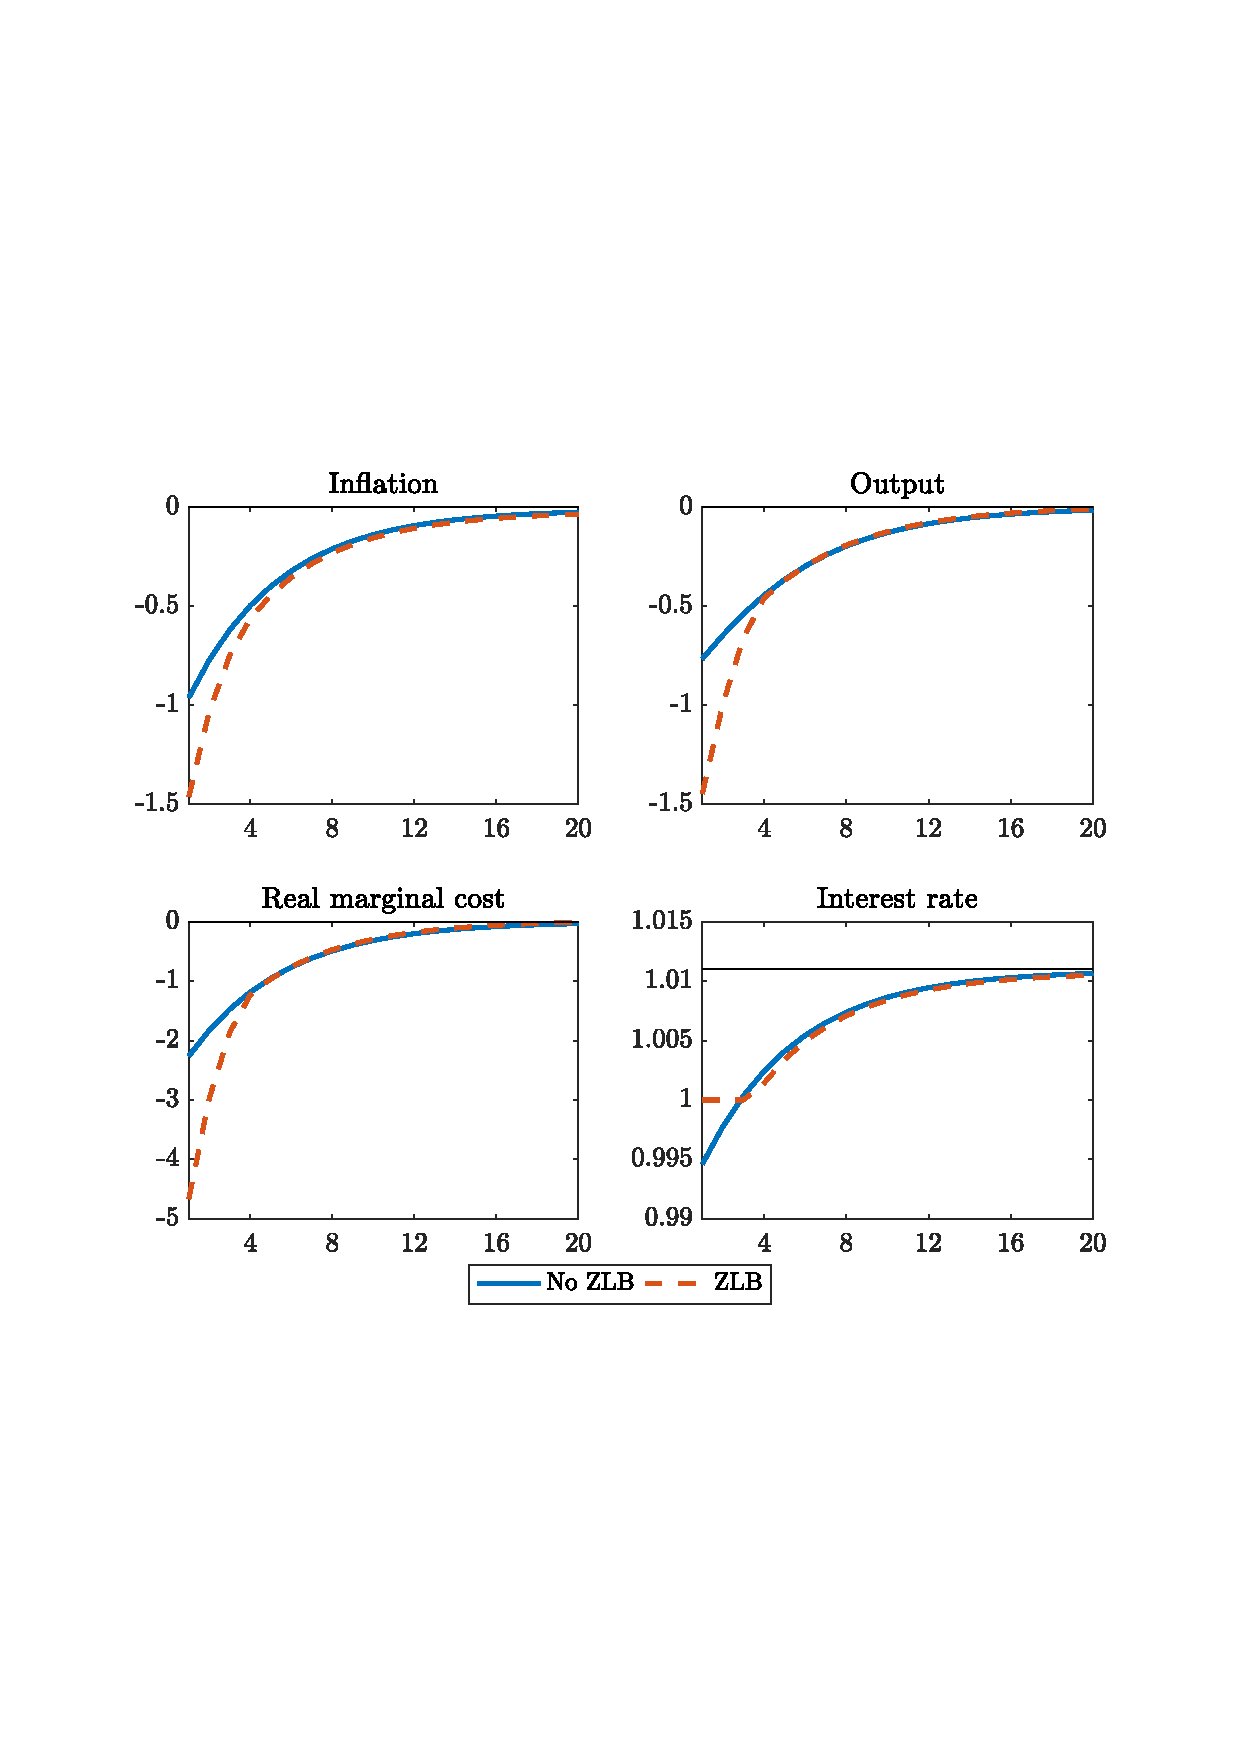
\includegraphics[scale=0.7]{irfLevel_pref}
%\end{figure}

\ctable[caption=Response of variables to a demand shock,
	center,
	label=fig:irfLevel_pref,
	figure,
	notespar,
	pos=H]{c}{{\sc Notes:} Blue solid lines corresponds to the baseline model when the zero lower bound is not considered. Red dashed lines activates the zero lower bound constraint. All responses to a negative demand shock, which corresponds to a one period increment in the discount factor. All responses plotted as percentage differences with respect to their steady state values, except interest rate which is plotted in gross terms.}
{
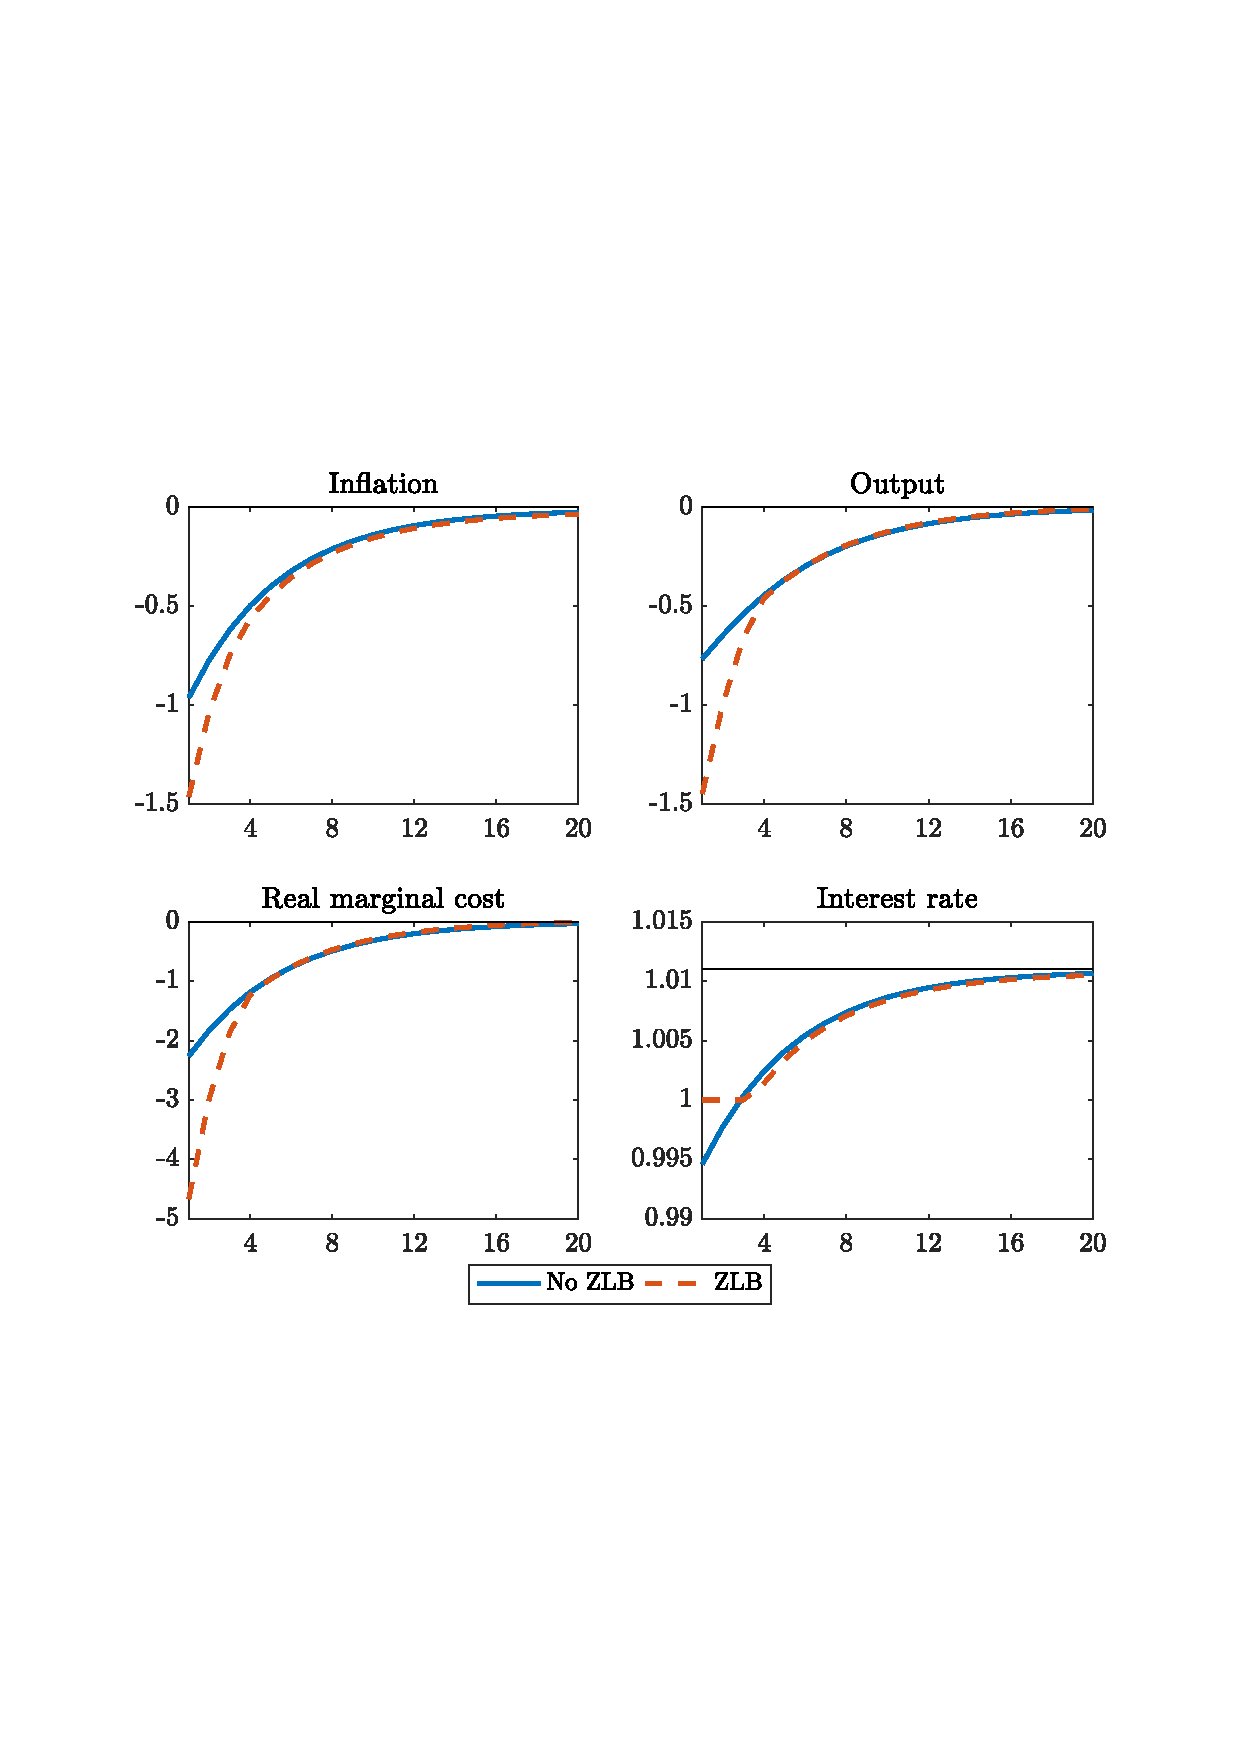
\includegraphics[scale=.6]{irfLevel_pref}
}

In Figure \ref{fig:irfExp_pref}, I present the response of private expectations of each variable, four and eight quarters ahead. To compute these expectations, at each step of the computation of the response of the system to the shock, I compute the one-step ahead expectation, given all possible realizations of the shock tomorrow (given by the quadrature nodes). With this, I recursively construct expectations up to the desired forecast horizon. Three interesting features emerge from the figure. First, the impact of the shock on expectations is larger on an horizon of four quarters than in an horizon of eight quarters. This is because the latter is closer to the long-run value for all the variables, hence, closer to the steady state. This is important for the discussion that comes later in the paper, in terms of measuring the effectiveness of policy: it depends on which horizon is the relevant for the decision making of private sector. Second, the impact of the shock on expectations is slightly larger in the case when the zero lower bound is considered in the economy, but the differences in general are modest. This implies that the zero lower bound plays a secondary role in the determination of expectations of the private sector, at least in the case of the impact of a large demand shock. Finally, note that the responses are in general smaller than the responses of variables in levels. In the case of inflation, we have a decrease of at most 0.5\%, while in output this decrease is at most of 0.4\%, in both cases for the four quarters horizon. For real marginal cost, we observe decreases between 0.5 and 1\%, while in the case of the interest rate, agents do not expect that it reaches the zero bound in the future, even considering that currently it reaches the lower bound for about four periods. Again, all this information is relevant because reflects that a policy that pretends to change expectations should expect modest effects.\footnote{The fact of modeling monetary policy with the help of a rule implies that the central bank is credible in its policy. With this, expectations are anchored, fact that is reflected in the small variation in expectations after the demand shock observed in Figure \ref{fig:irfExp_pref}.}

%\begin{figure}[H]
%	\centering
%	\caption{Response of variables in expectation to a demand shock}\label{fig:irfExp_pref}
%	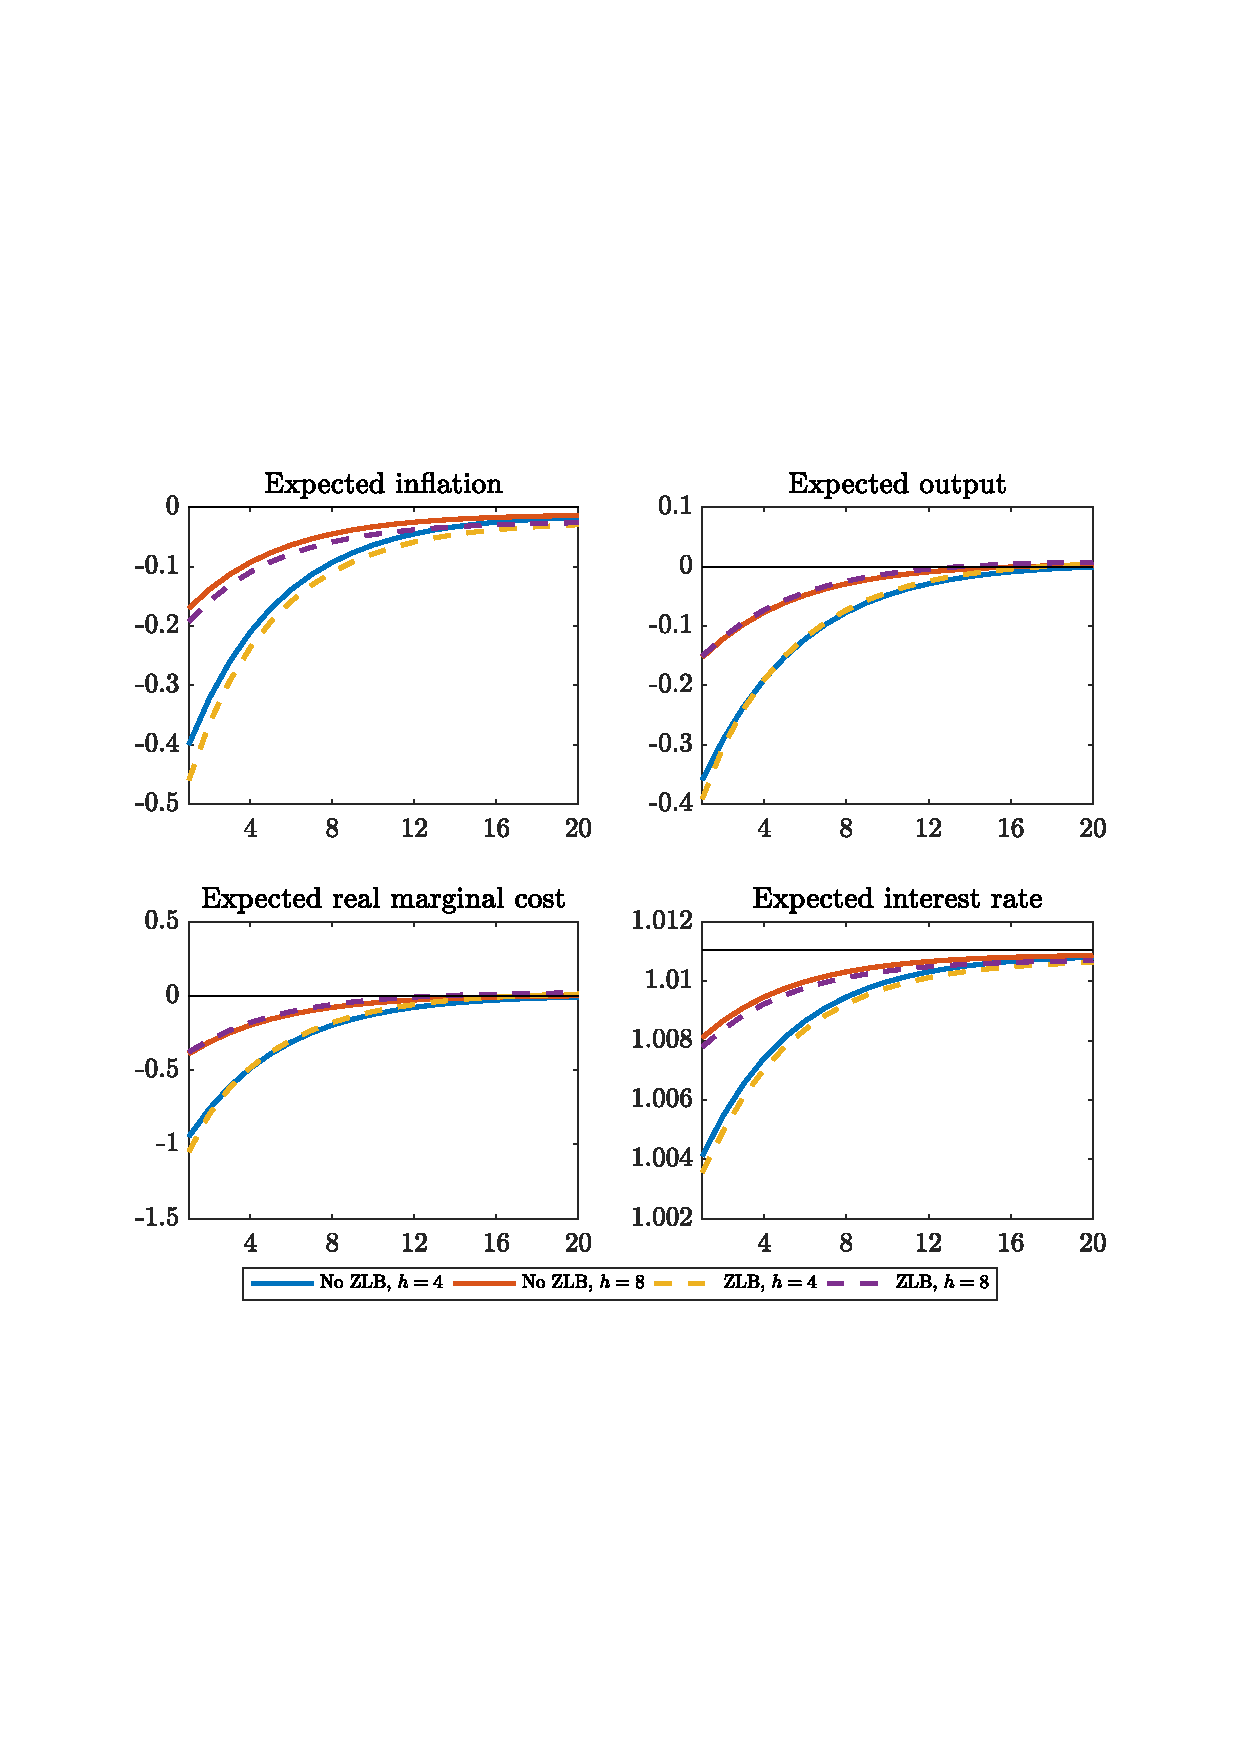
\includegraphics[scale=0.7]{irfExp_pref}
%\end{figure}

\ctable[caption=Response of variables in expectation to a demand shock,
	label=fig:irfExp_pref,
	figure,
	notespar,
	pos=H]{c}{{\sc Notes:} Blue and red solid lines corresponds to the baseline model when the zero lower bound is not considered, for horizons of four and eight quarters, respectively. Yellow and purple dashed lines activates the zero lower bound constraint, for horizons of four and eight quarters, respectively. Expectations are computed as recursive one-step-ahead forecast over simulations. All responses to a negative demand shock, which corresponds to a one period increment in the discount factor. All responses plotted as percentage differences with respect to their steady state values, except interest rate which is plotted in gross terms.}
{
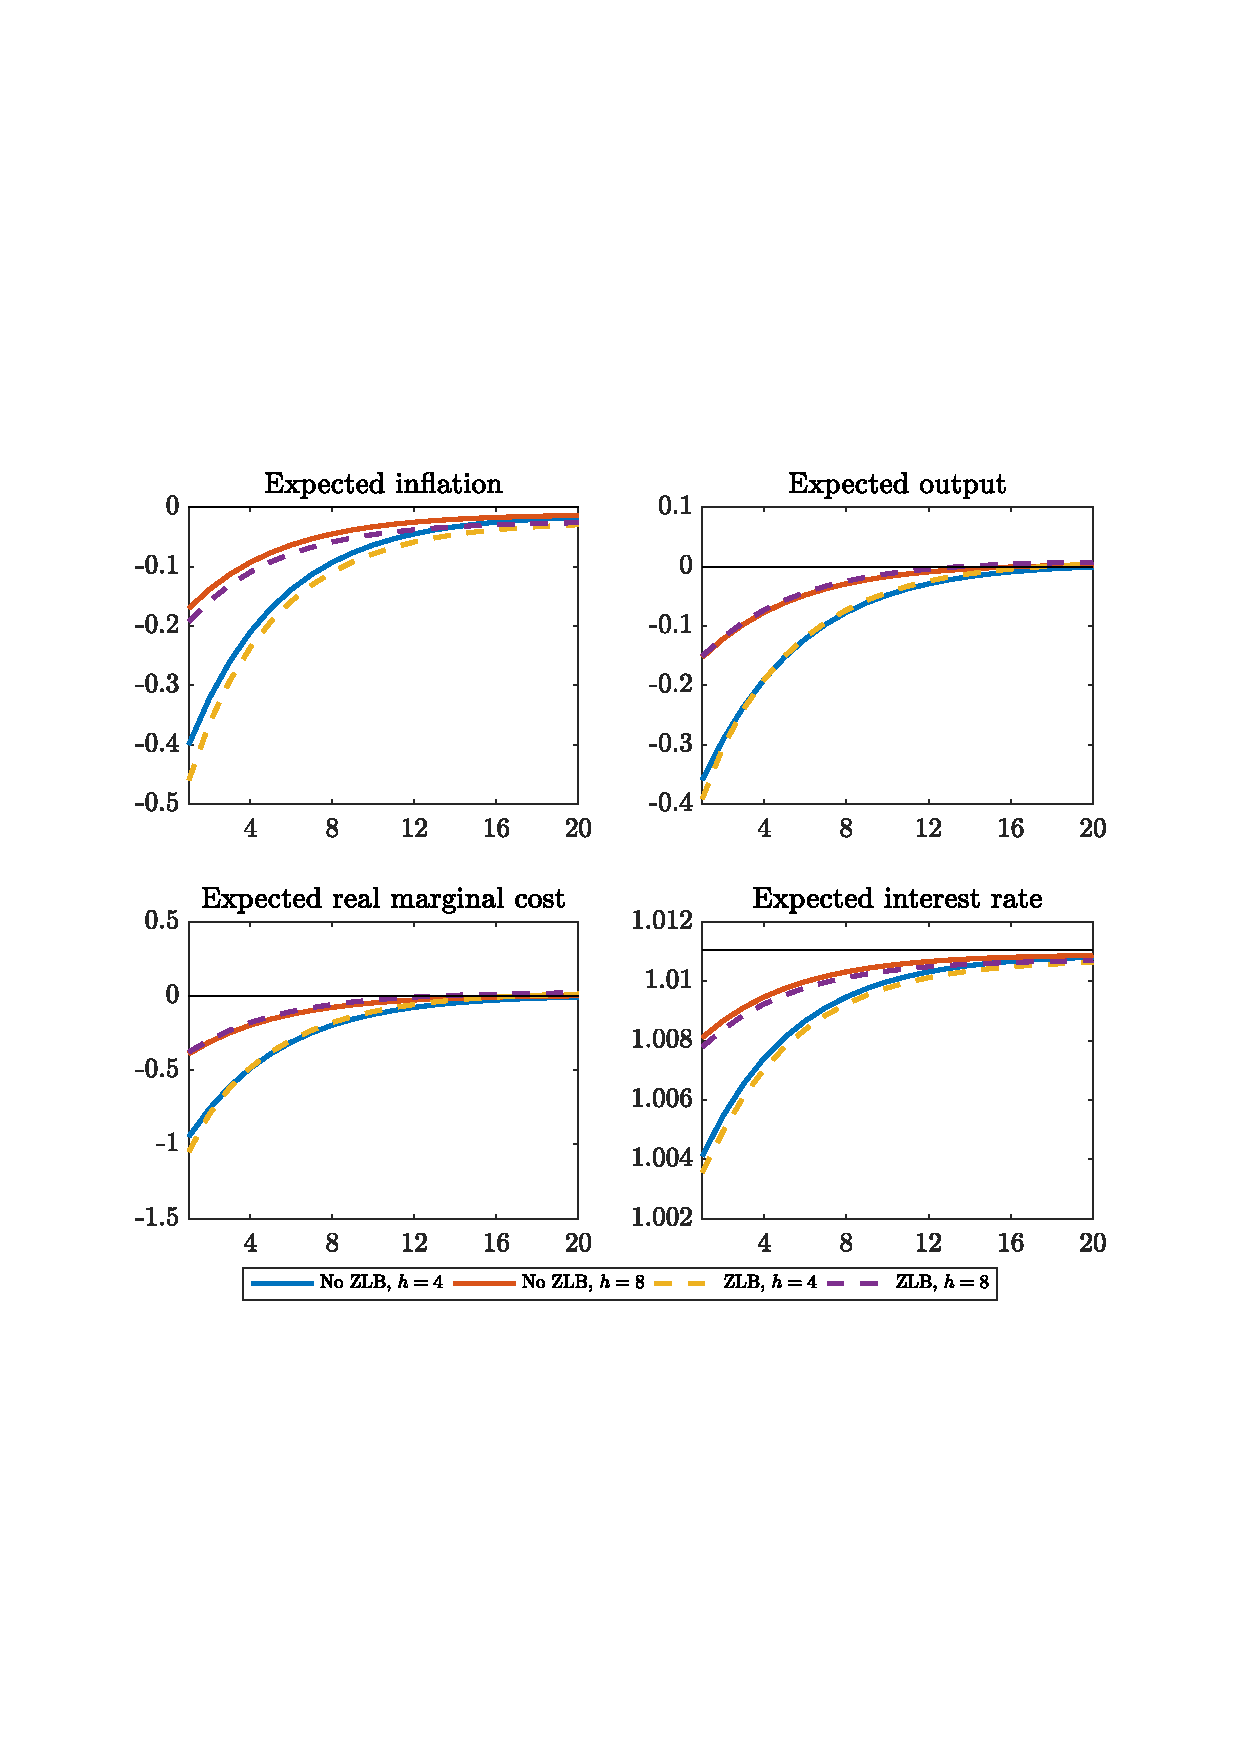
\includegraphics[scale=.6]{irfExp_pref}
}

\subsection{The effect of pseudo forward guidance}

\paragraph{Comparing the standard Taylor rule with the extended one.} Once I have compared the responses of the model with and without the zero lower bound, I proceed to analyze the effect that the backward looking or pseudo forward guidance component has on the economy. In order to do this, I compare the impulse-response functions of the model to the same shock of previous section, but comparing the case with zero lower bound and no forward guidance channel, with the case when the forward guidance is present (and also the zero lower bound) using past output and past inflation as alternatives for the authority. For these comparisons, I use the model with a forward guidance parameter $\phi_{FG}=1$.\footnote{To make the comparison fair between both specifications, in the case of zero lower bound without forward guidance I set to $\phi_{FG}=0$. This means that the forward guidance policy assumes an specific value of zero but it is present in the model. In this case, the policy function for different values of the forward guidance variable are exactly the same and the only variation is between values of the discount factor.}

In Figure \ref{fig:irfCompLevel_pref}, I plot the impulse-responses for variables in levels. As in previous section, I plot the percentage difference of the each variables with respect to its steady-state value, except for interest rate which is in gross terms. From this figure, I can distinguish three interesting results. First, the decrease in all variables is considerably smaller than in the case without the extra forward guidance term. In the case of inflation, now we have a decrease of about 0.5\%, which is one third relative to the case with no extra variables in the policy rule. In the case of output, the decrease is about 0.7\%, which is a half of the value in previous exercise. For real marginal cost we observe a decrease of 2\% against the 4.5\% in the case without forward guidance policy. Second, there is no difference between applying the policy considering past output or past inflation. This is because no matter which macroeconomic variable is considered, this will summarize all the relevant information about the state of the economy in previous period.\footnote{I also evaluated a third modification of the policy which is to include the past value of interest rate. This version does not allow to consider large enough values for the forward guidance parameter because it generate explosive paths for the policy rule given its autoregressive structure. For this lack of comparability, I discarded these results for current presentation.} Finally, note that with the presence of the forward guidance policy, the zero lower bound is reached just in one period and the level of interest rates are slightly larger than without the modified policy. The authority now takes into account, not only the current level of economic conditions, but also their past level. Because the central bank internalizes the effect that its actions have on the equilibrium of the economy, now, under the modified policy, decreases the interest rate but up to a level slightly above the zero rate, such that avoids a deflationary process of the economy. However, note that this decrease is on impact larger than zero, but in the second period reaches the zero lower bound just for that period, to then increase the level of the policy instrument again during the following quarters. This implies that the authority considers that the economy requieres and additional impulse and gives it during the second period after the shock, to help the recovery of the real side of the economy. This is consistent with the slope change in second panel (output), where the recovery between periods one and two is larger than in the rest of periods. The important thing here is that the authority uses the zero lower bound on its favor to push the economy out of the recession and not as a consequence of keeping the interest rate too low for too long.

%\begin{figure}[H]
%	\centering
%	\caption{Comparison of the response of variables between the model with and without forward guidance}\label{fig:irfCompLevel_pref}
%	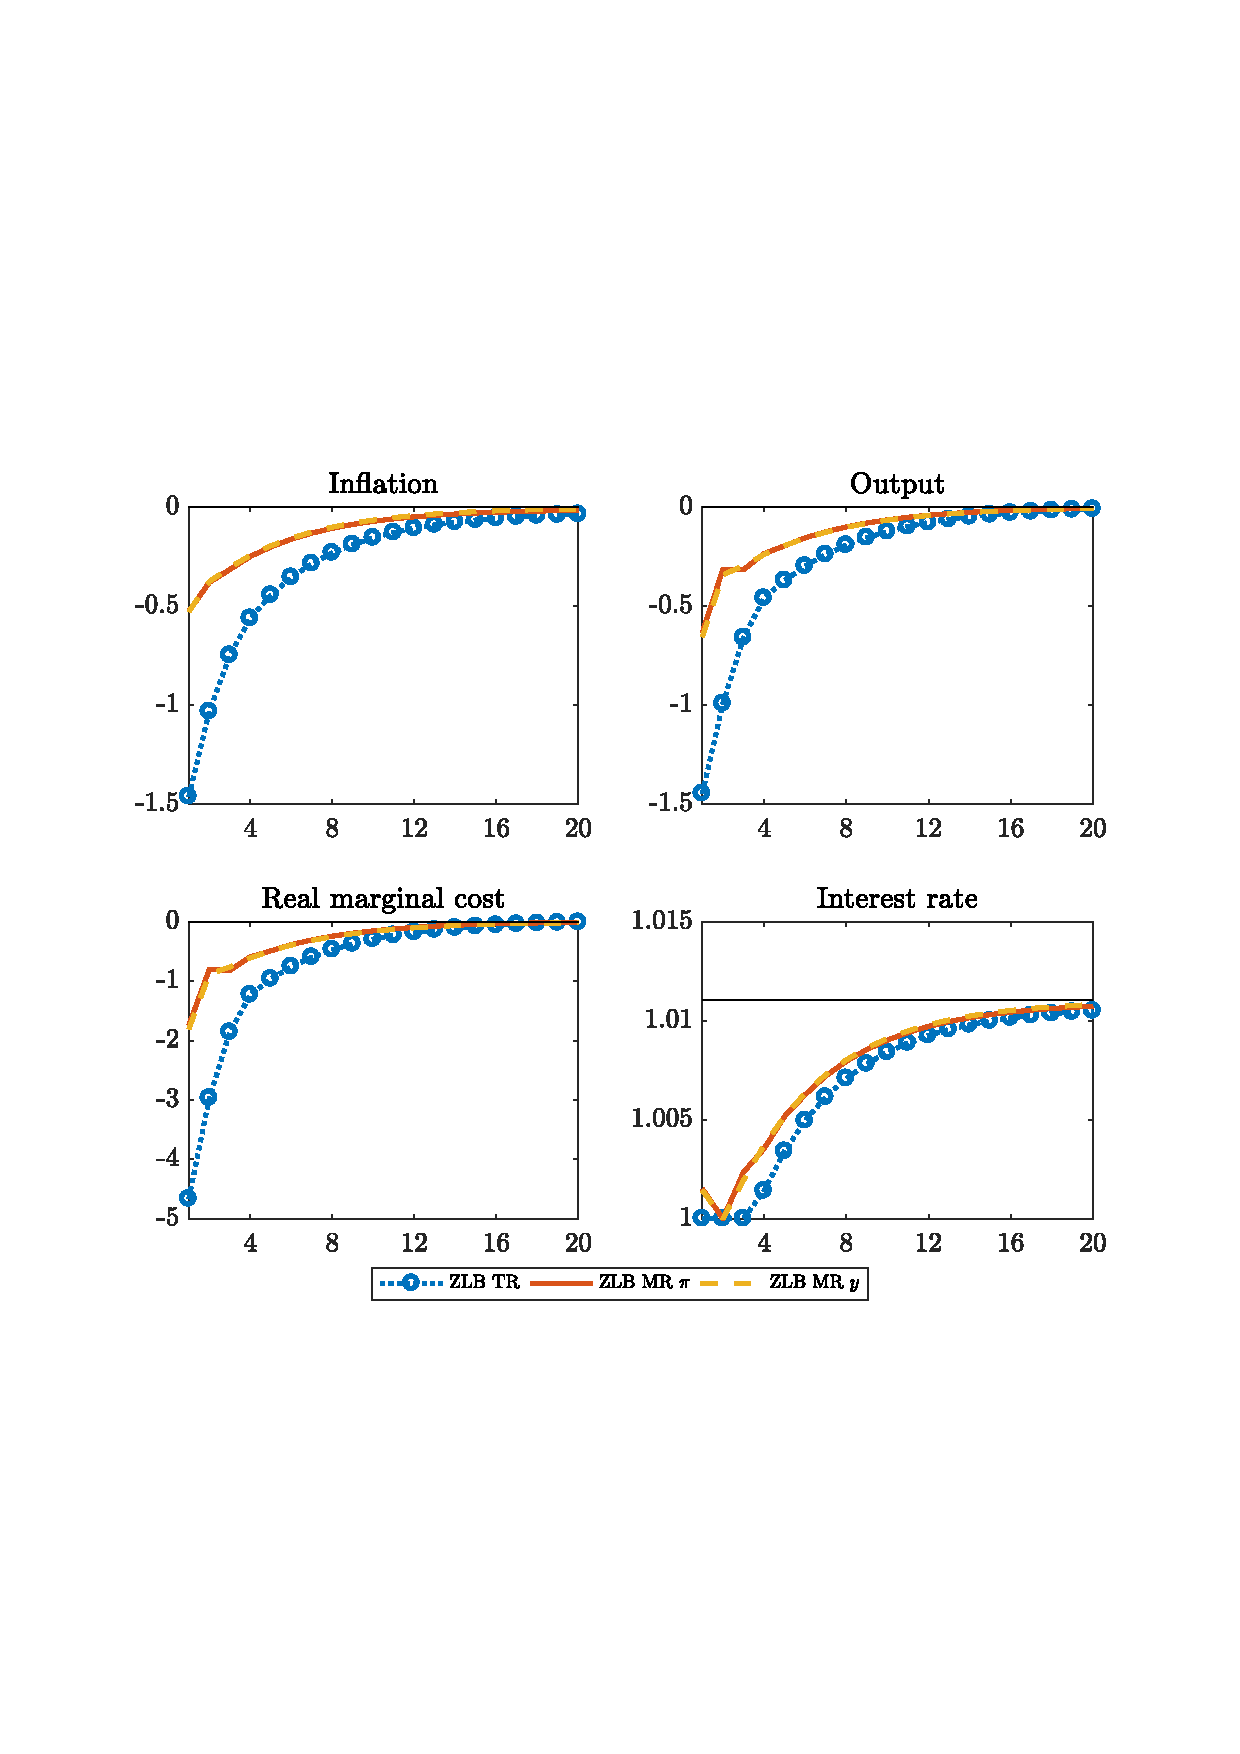
\includegraphics[scale=0.7]{irfCompLevel_pref}
%\end{figure}

\ctable[caption=Comparison of the response of variables between the model with and without forward guidance,
	label=fig:irfCompLevel_pref,
	figure,
	notespar,
	pos=H]{c}{{\sc Notes:} All lines are responses of variables in a model where the zero lower bound constraint is active. Blue dotted line corresponds to the response of the respective variable in a model where the interest rate determination does not include past macroeconomic variables. Red continuous line corresponds to the response in a model where the interest rate determination includes past inflation. Yellow dashed line corresponds to the response in a model where the interest rate determination includes past inflation. All responses to a negative demand shock, which corresponds to a one period increment in the discount factor. All responses plotted as percentage differences with respect to their steady state values, except interest rate which is plotted in gross terms.}
{
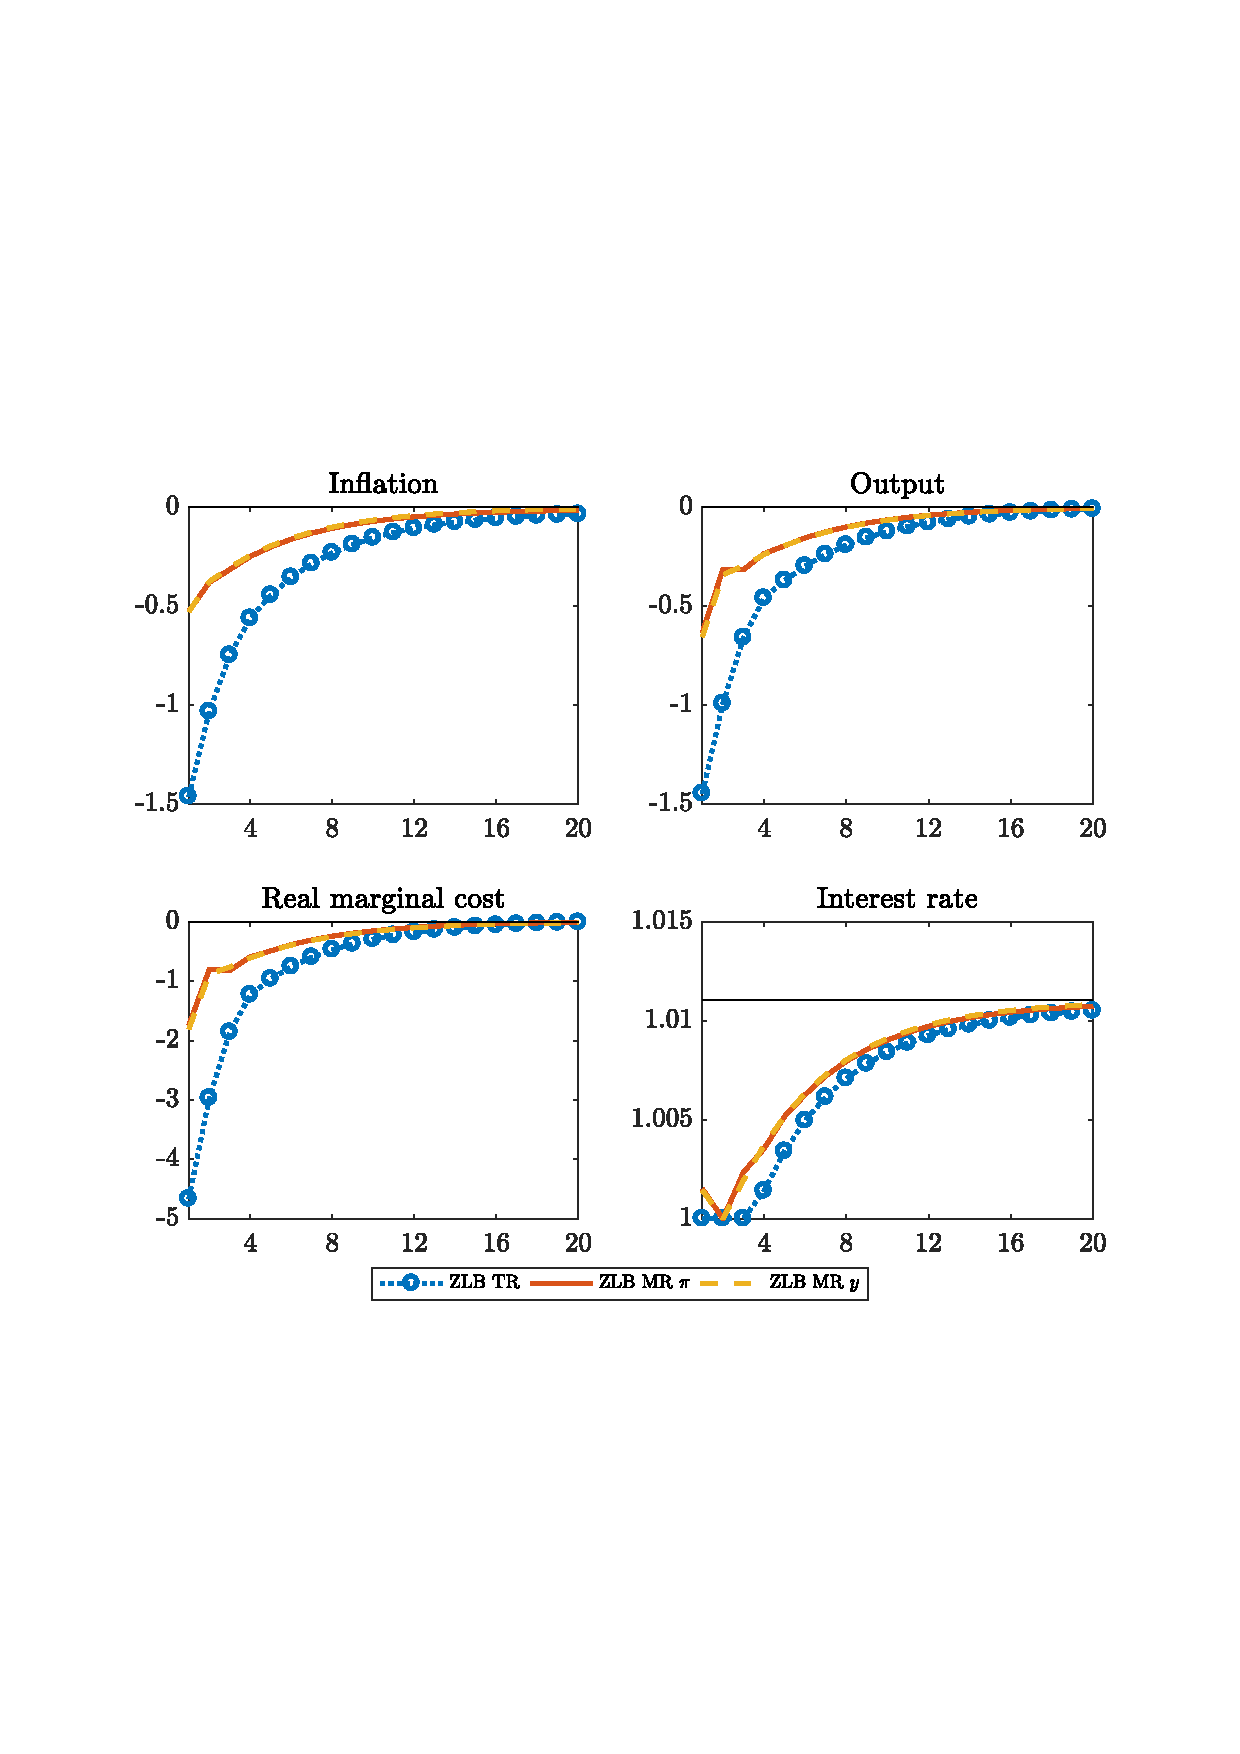
\includegraphics[scale=.6]{irfCompLevel_pref}
}

In Figures \ref{fig:irfCompExp4_pref} and \ref{fig:irfCompExp8_pref}, I present the responses of expectations four and eight quarters ahead respectively. Three features are important here. First, responses using the extended Taylor rule generates smaller decreases in expectation for all variables in the system than in the case without these extensions. This generates a departure respect to the benchmark case with respect to expectations, which are modified by in a smaller magnitude. Second, these gains are more notably experienced in the case of expectations four quarters ahead, where the impact of the demand shock is larger. In this case, gains for inflation, output and real marginal costs are about 50\% on impact, while are much more modest in the case of expected interest rate. Third, there is no distinction between using inflation or output as the extra element in the Taylor rule at any horizon, which was already noticed in the case of variables in levels (figure \ref{fig:irfCompLevel_pref}).

%\begin{figure}[H]
%	\centering
%	\caption{Comparison of the response of variables between the model with and without forward guidance for expected variables four quarters ahead}\label{fig:irfCompExp4_pref}
%	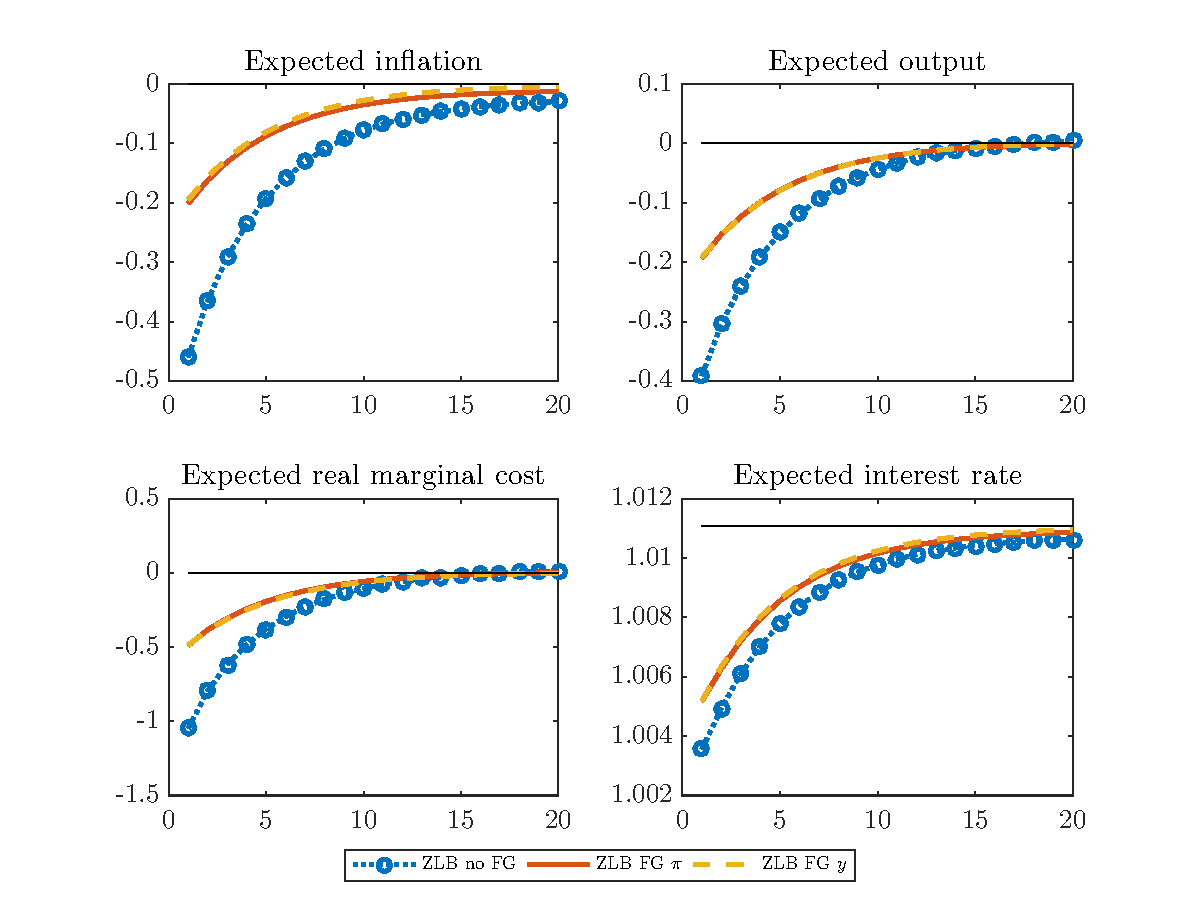
\includegraphics[scale=0.7]{irfCompExp4_pref}
%\end{figure}

\ctable[caption=Comparison of the response of variables between the model with and without forward guidance for expected variables four quarters ahead,
	label=fig:irfCompExp4_pref,
	figure,
	notespar,
	pos=H]{c}{{\sc Notes:} All lines are responses of variables in a model where the zero lower bound constraint is active. Blue dotted line corresponds to the response of the respective variable in a model where the interest rate determination does not include past macroeconomic variables. Red continuous line corresponds to the response in a model where the interest rate determination includes past inflation. Yellow dashed line corresponds to the response in a model where the interest rate determination includes past inflation. Expectations are computed as recursive one-step-ahead forecast over simulations. All responses to a negative demand shock, which corresponds to a one period increment in the discount factor. All responses plotted as percentage differences with respect to their steady state values, except interest rate which is plotted in gross terms.}
{
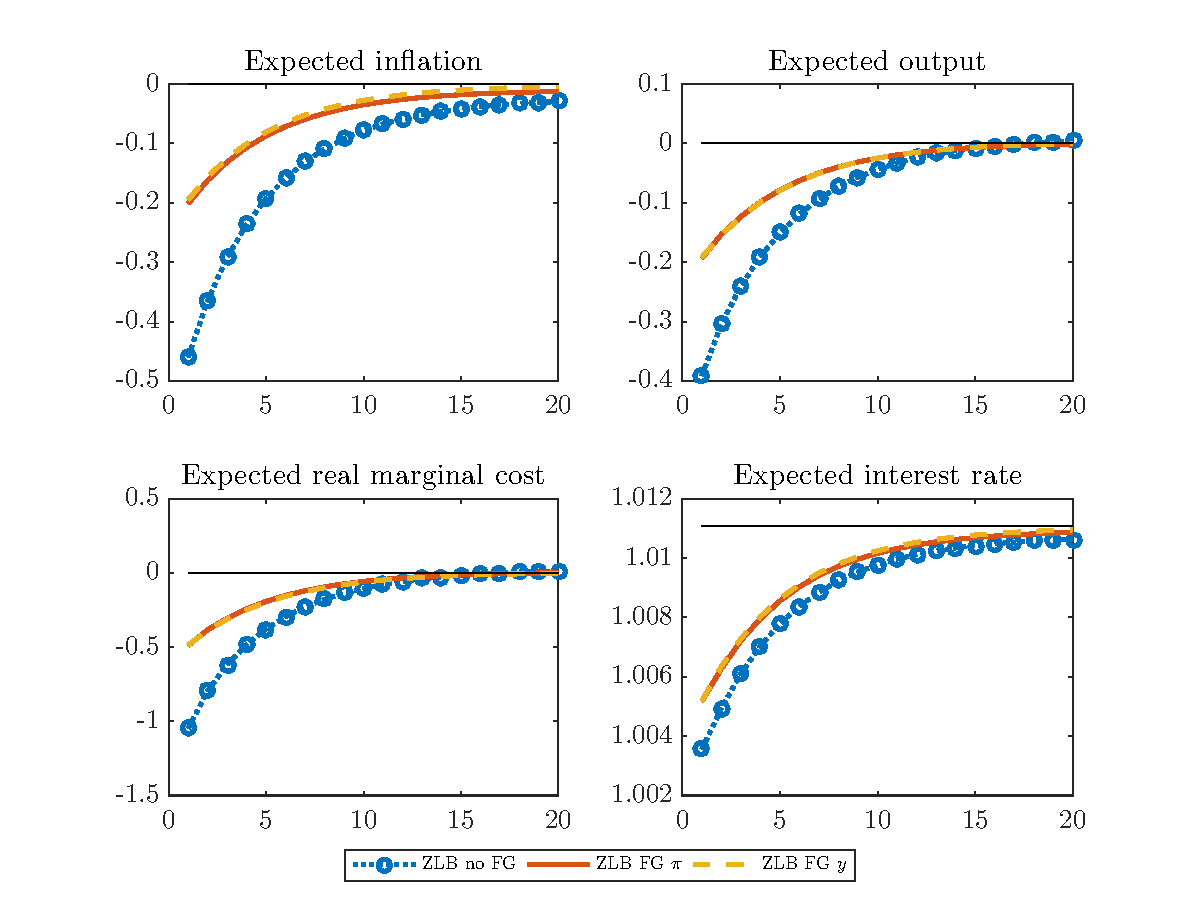
\includegraphics[scale=.6]{irfCompExp4_pref}
}

%\begin{figure}[H]
%	\centering
%	\caption{Comparison of the response of variables between the model with and without forward guidance for expected variables eight quarters ahead}\label{fig:irfCompExp8_pref}
%	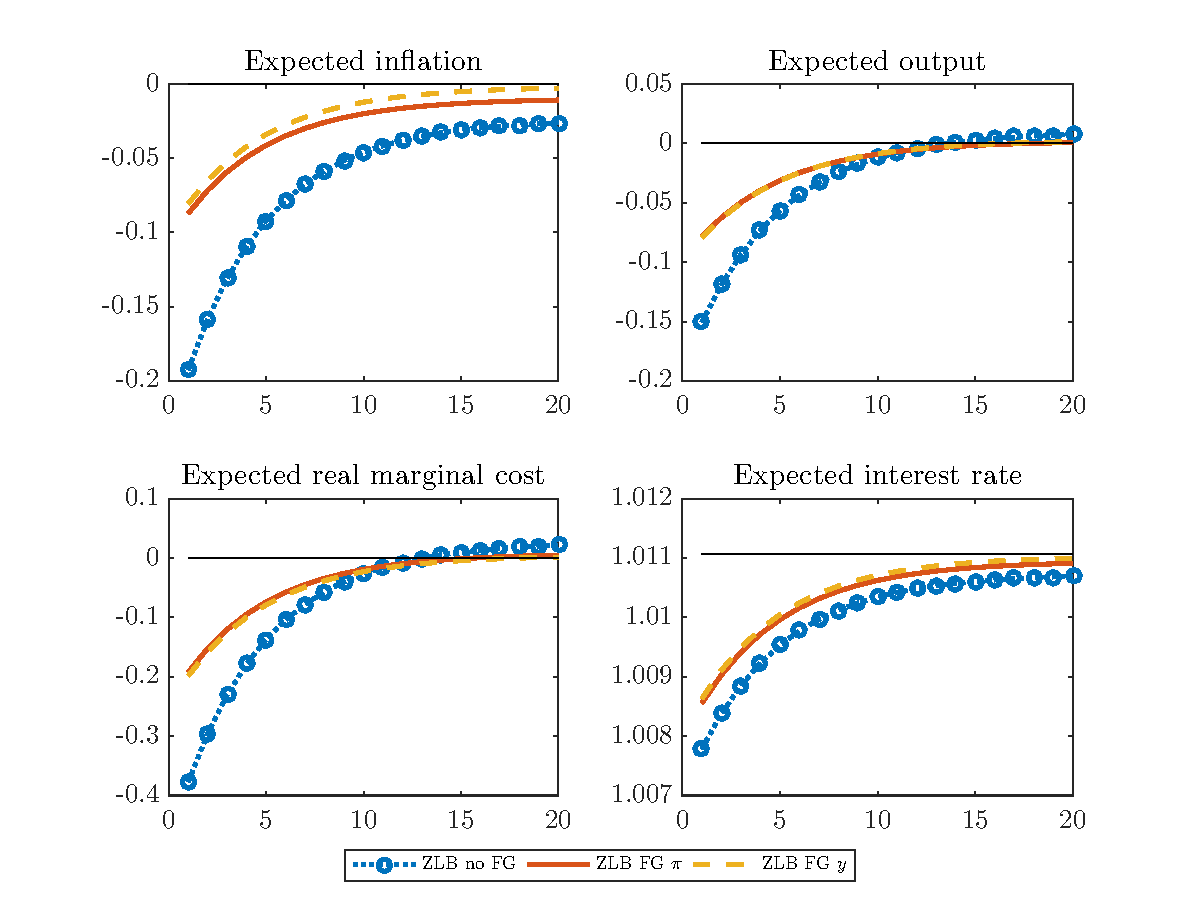
\includegraphics[scale=0.7]{irfCompExp8_pref}
%\end{figure}

\ctable[caption=Comparison of the response of variables between the model with and without forward guidance for expected variables eight quarters ahead,
	label=fig:irfCompExp8_pref,
	figure,
	notespar,
	pos=H]{c}{{\sc Notes:} All lines are responses of variables in a model where the zero lower bound constraint is active. Blue dotted line corresponds to the response of the respective variable in a model where the interest rate determination does not include past macroeconomic variables. Red continuous line corresponds to the response in a model where the interest rate determination includes past inflation. Yellow dashed line corresponds to the response in a model where the interest rate determination includes past inflation. Expectations are computed as recursive one-step-ahead forecast over simulations. All responses to a negative demand shock, which corresponds to a one period increment in the discount factor. All responses plotted as percentage differences with respect to their steady state values, except interest rate which is plotted in gross terms.}
{
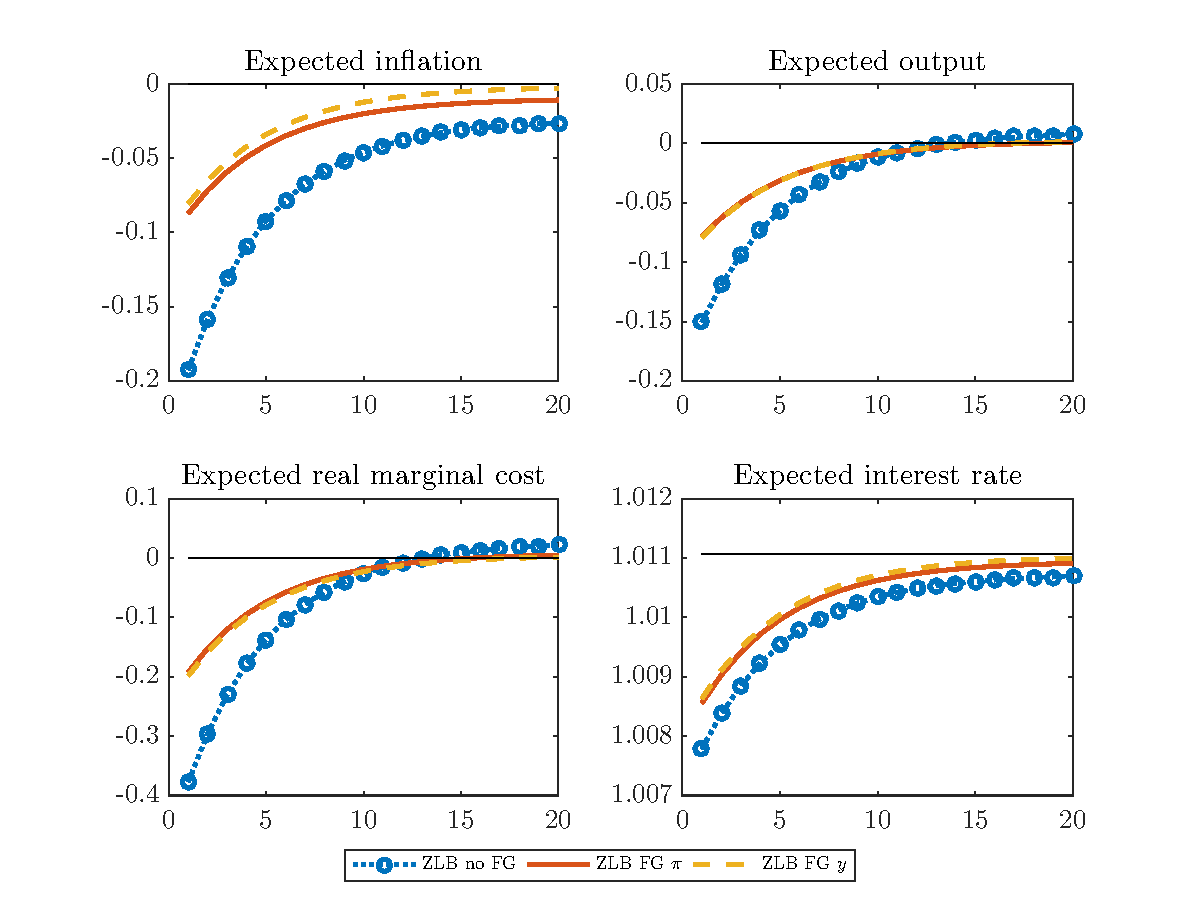
\includegraphics[scale=.6]{irfCompExp8_pref}
}

\paragraph{Comparing different degrees of the extended Taylor rule.} To study in more depth the power of the extended Taylor rule, I compare the responses of the economy using different degrees of relevance of past macroeconomic variables for current interest rate determination. To do this, I present two exercises. First, I compare the impulse-response function using two extreme values for the $\phi_{FG}$ parameter: 0.5 and 2. In the former case, past variables are at most as relevant for current policy as current variables, while in the latter are even more important than current variables. I just present these two values because the responses are monotone on the degree of persistence of the macroeconomic variable in the rule, so all other values are incorporated in between these responses. In this regard, this exercise shows a lower and upper bound for each possible response. For this exercise, I present both cases using past output and past inflation as relevant variables. In the second exercise, I present the long-run distribution under different configurations of the forward guidance parameter to present the relative gains of the rules.

In Figure \ref{fig:irfCompDegreeLevel_pref}, I present the responses of the macroeconomic variables for different configurations of the extended Taylor rule. For each case, the zero lower bound is present in the model. The first set of curves use past output as the past variable relevant for policy, with changes in the level of importance of this variable from 0.5 to 2. The second set of curves does the same comparison but using past inflation as the key indicator. As in the case presented in the previous section, we note that in general there is no relevant difference between using past output or past inflation as the variable of interest for the authority. The key component is the importance that the authority gives to this variable ($\pi_{FG}$ coefficient). For simplicity, I will do the comparison among the different degrees of sensitivity for the authority just for the case of output in the Taylor rule, given previous evidence that illustrates that responses does not vary much when the Taylor rule uses past inflation. In general we can see that the gains of having a more aggressive rule--for variables in level--are relevant. In the case of inflation, by using a rule with $\phi_{FG}=2$, the central bank diminishes the impact of the shock from -0.8 to -0.4\%, where this former number is when the central bank uses the less aggressive rule ($\phi_{FG}=0.5$). In the case of output, the figure shows gains from -0.8 to -0.6\%. An interesting element of this figure is that the convergence of the more aggressive rule is oscillatory when past output is taken into account. This is the main difference with a rule that uses past inflation: in this latter case the convergence to the long-run equilibrium is smooth, while in the case of past output as the relevant indicator we observe oscillations along the path. For real marginal cost the gains after the shock goes from -2.5 to -1.5\%. Taking $\phi_{FG}=0.5$ as the baseline results, the gains experienced by increasing the sensitivity of the authority to $\phi_{FG}=2$ fluctuates between 30 to 100\% on impact. Finally, for the interest rate determination, we observe that there is no difference between the degree of importance or the variable employed: the interest rate is reduced on impact, while the zero lower bound is attained on the second period. After this, the central bank increases monotonically the interest rate to its long-run value. The only difference is a small discrepancy between the impact effect of the rules, but this is negligible.

%\begin{figure}[H]
%	\centering
%	\caption{Comparison between different intensities in the extended Taylor rule: impulse-responses}\label{fig:irfCompDegreeLevel_pref}
%	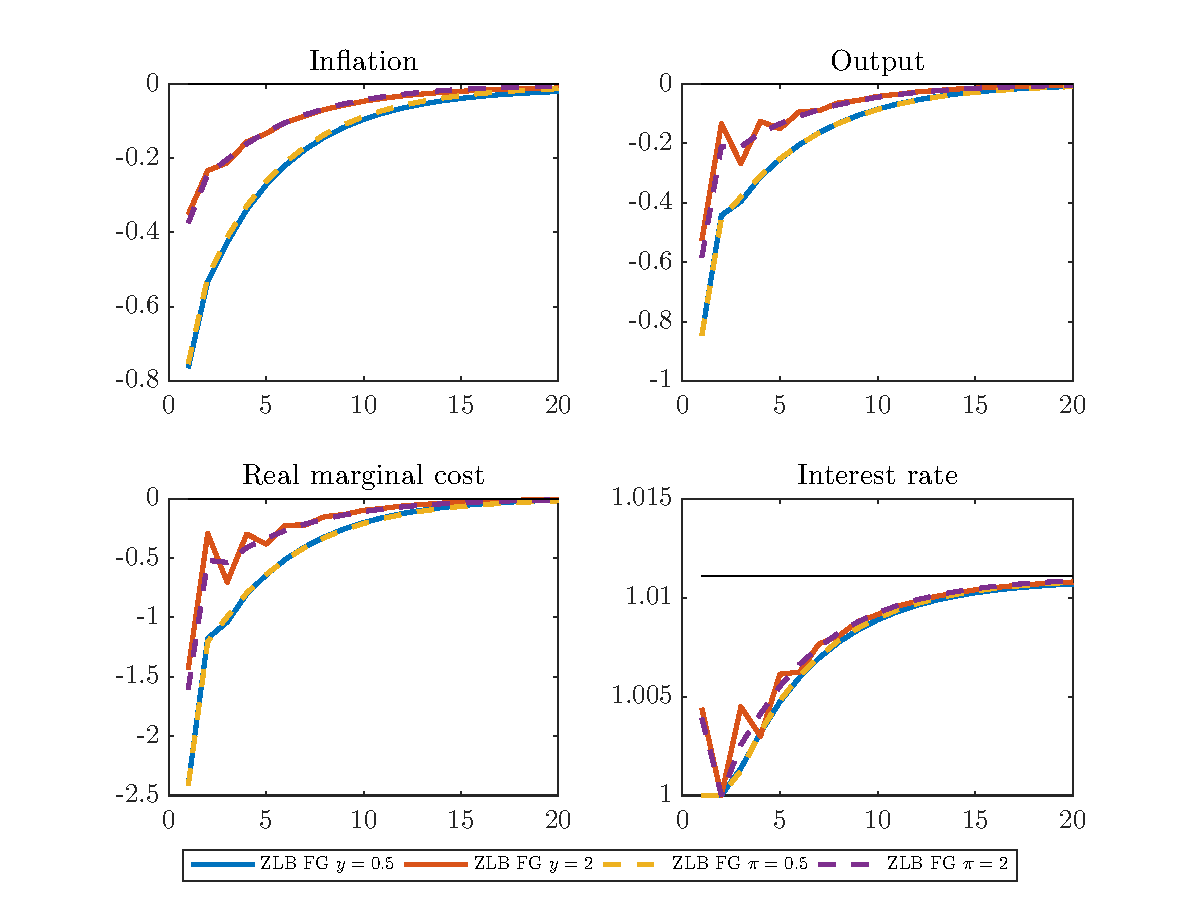
\includegraphics[scale=0.7]{irfCompDegreeLevel_pref}
%\end{figure}

\ctable[caption=Comparison between different intensities in the extended Taylor rule: impulse-responses,
	label=fig:irfCompDegreeLevel_pref,
	figure,
	notespar,
	pos=H]{c}{{\sc Notes:} Blue and red solid lines corresponds to the model when the central bank sets the interest rate using current inflation and output and also past output, where the level of importance of this last variables is of 0.5 and 2, respectively. Yellow and purple dashed lines corresponds to the model when the central bank sets the interest rate using current inflation and output and also past output, where the level of importance of this last variables is of 0.5 and 2, respectively. All responses to a negative demand shock, which corresponds to a one period increment in the discount factor. All responses plotted as percentage differences with respect to their steady state values, except interest rate which is plotted in gross terms.}
{
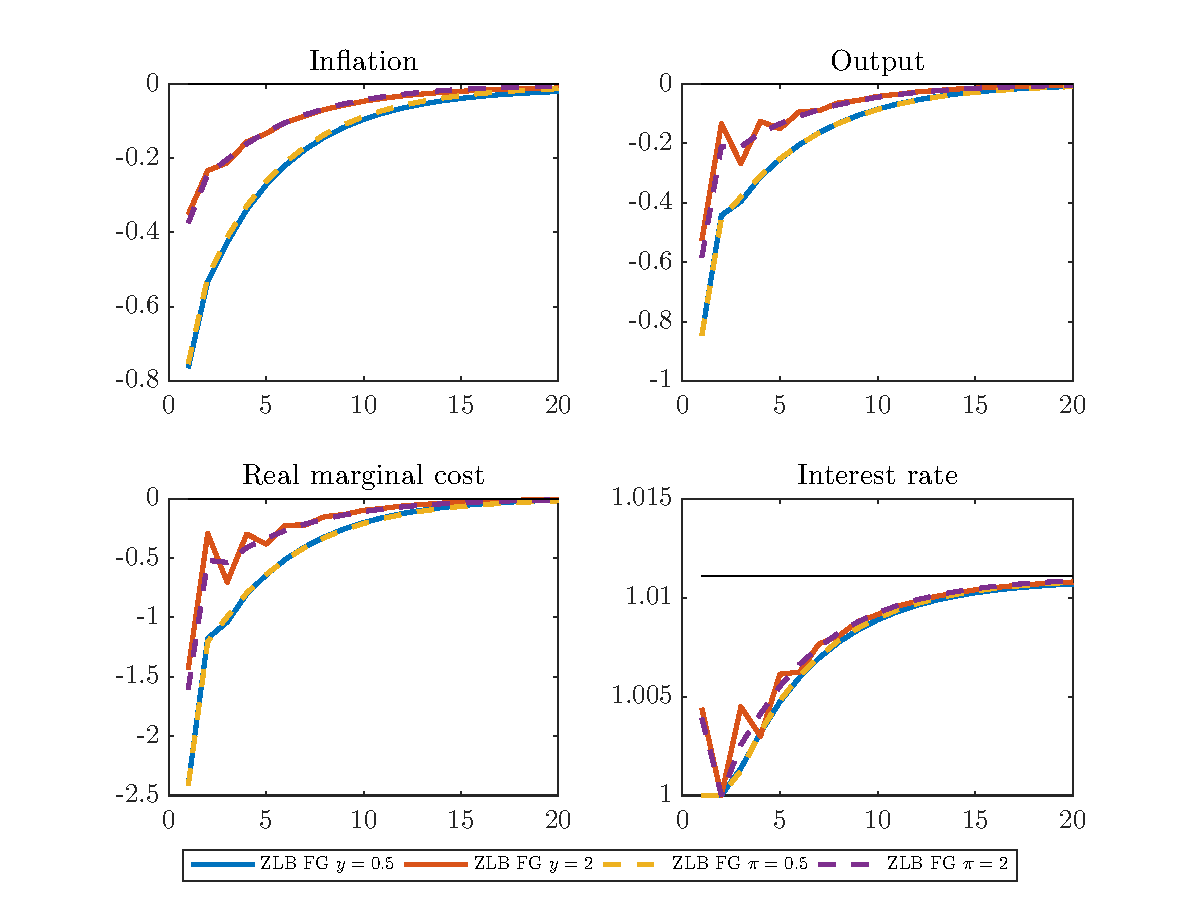
\includegraphics[scale=.6]{irfCompDegreeLevel_pref}
}

In Figure \ref{fig:irfCompDegreeExp4_pref}, I show the responses of expectations four periods ahead. In all cases but the interest rate, there are differences in the reaction of expectations of using a more aggressive rule. These gains are, on impact, of 0.2, 0.1 and 0.2\% for inflation, output and real marginal cost, respectively. This result is relevant because the authority must take into account how its policy will affect private expectations and how this will modify the decision making process of consumers and firms. The figure suggest that the more aggressive the policy, the less affected are the expected values, which is in line with well anchored expectations by private agents and a credible monetary policy. In the case of interest rate, there is no difference in the reaction of expectation to the shock.

%\begin{figure}[H]
%	\centering
%	\caption{Comparison between different intensities in the extended Taylor rule for expectations four quarters ahead: impulse-responses}\label{fig:irfCompDegreeExp4_pref}
%	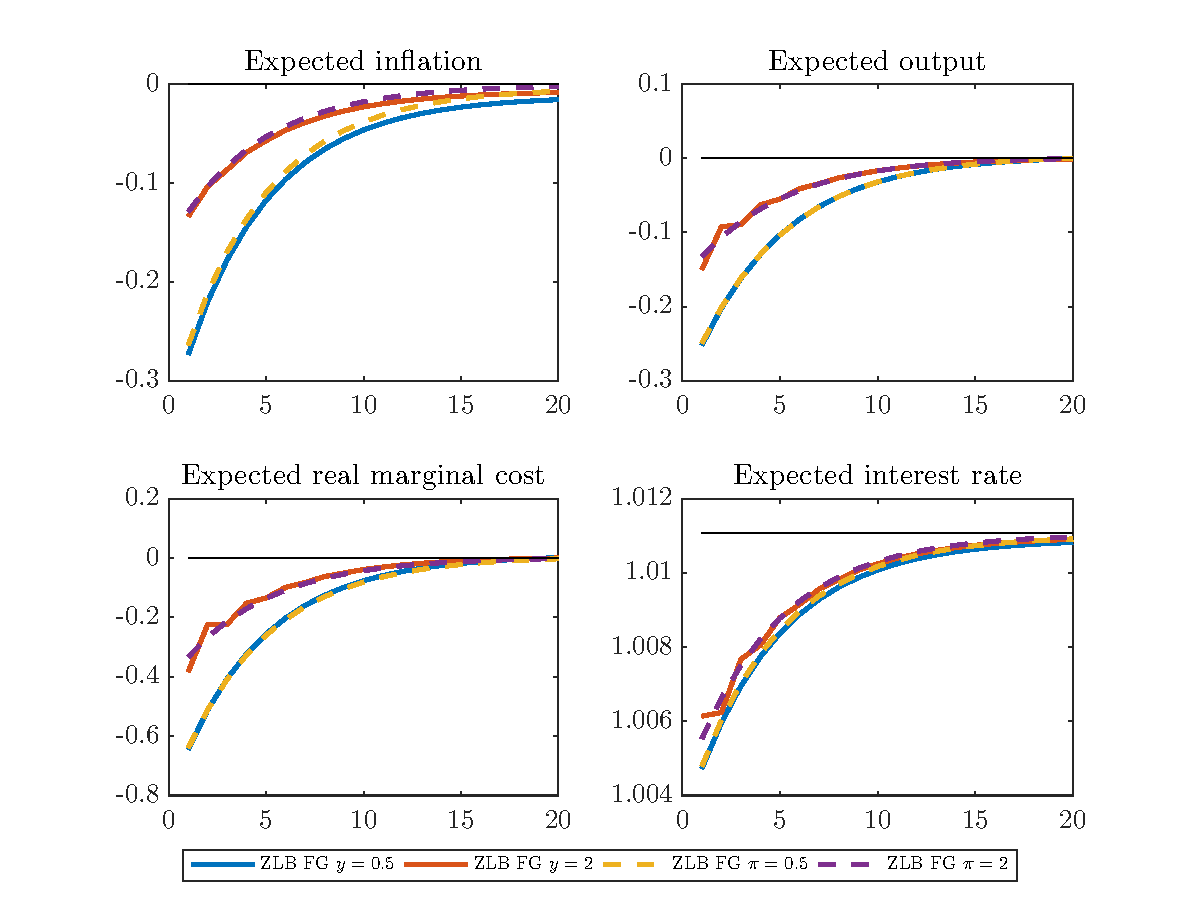
\includegraphics[scale=0.7]{irfCompDegreeExp4_pref}
%\end{figure}

\ctable[caption=Comparison between different intensities in the extended Taylor rule for expectations four quarters ahead: impulse-responses,
	label=fig:irfCompDegreeExp4_pref,
	figure,
	notespar,
	pos=H]{c}{{\sc Notes:} Blue and red solid lines corresponds to the model when the central bank sets the interest rate using current inflation and output and also past output, where the level of importance of this last variables is of 0.5 and 2, respectively. Yellow and purple dashed lines corresponds to the model when the central bank sets the interest rate using current inflation and output and also past output, where the level of importance of this last variables is of 0.5 and 2, respectively. Expectations are computed as recursive one-step-ahead forecast over simulations. All responses to a negative demand shock, which corresponds to a one period increment in the discount factor. All responses plotted as percentage differences with respect to their steady state values, except interest rate which is plotted in gross terms.}
{
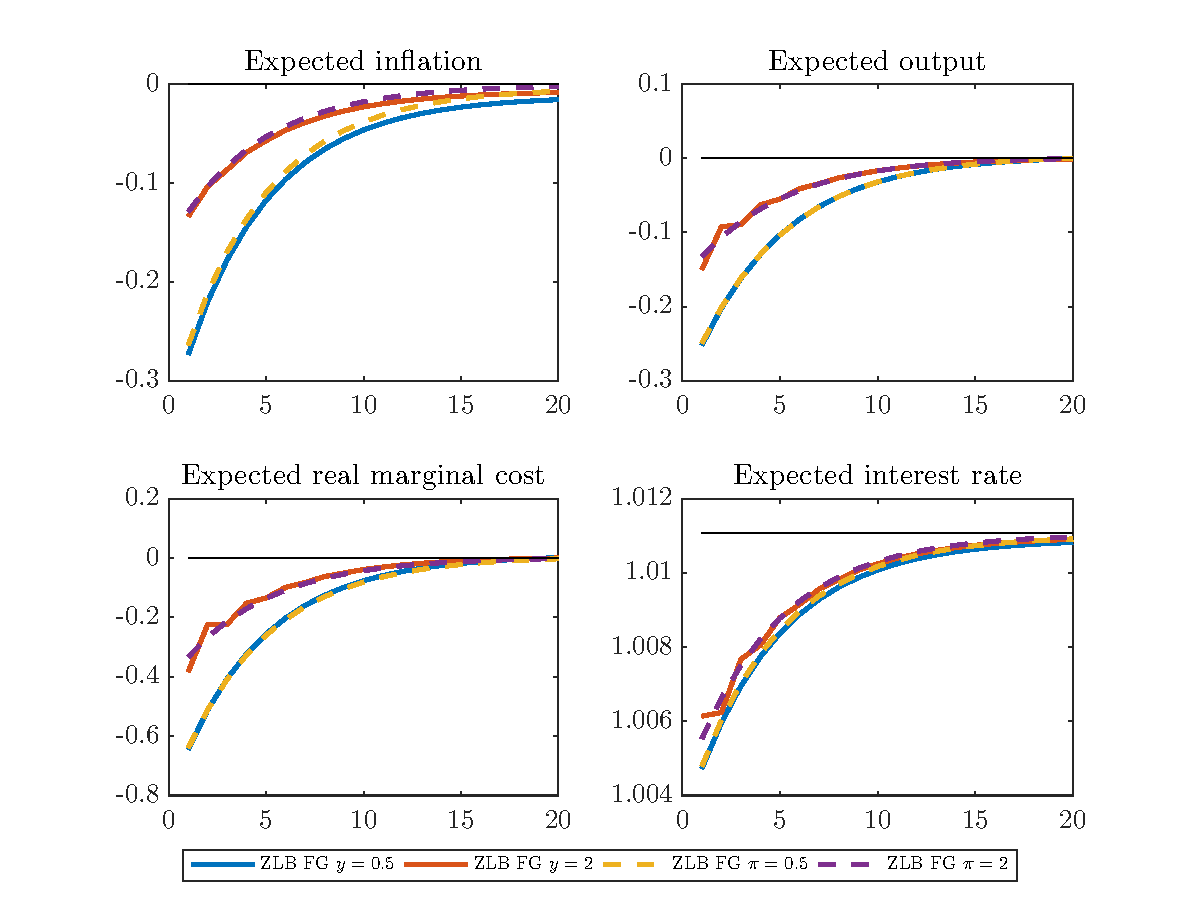
\includegraphics[scale=.6]{irfCompDegreeExp4_pref}
}

Finally, in Figure \ref{fig:irfCompDegreeExp8_pref}, I present the responses of expectations eight quarters ahead. Again, analyzing the differences in expectations between two different horizons is a relevant exercise because some decisions are taken considering a shorter horizon than others and monetary authority should take this into account when doing policy. Three elements are important here. First, the responses of expectations are smaller than in the four periods horizon case. Given that eight periods is closer to the long-run than four periods, this is a reasonable result. Second, the same differences between the level of $\phi_{FG}$ parameter are observed, where the more aggressive rules produce smaller responses, except for the case of interest rate. Third, unlike previous cases, there exist minor differences between using past output and past inflation for the case of expected inflation. In particular, the decrease in expected inflation is smaller when past inflation is used by the authority. However, these differences are small.

%\begin{figure}[H]
%	\centering
%	\caption{Comparison between different intensities in the extended Taylor rule for expectations eight quarters ahead: impulse-responses}\label{fig:irfCompDegreeExp8_pref}
%	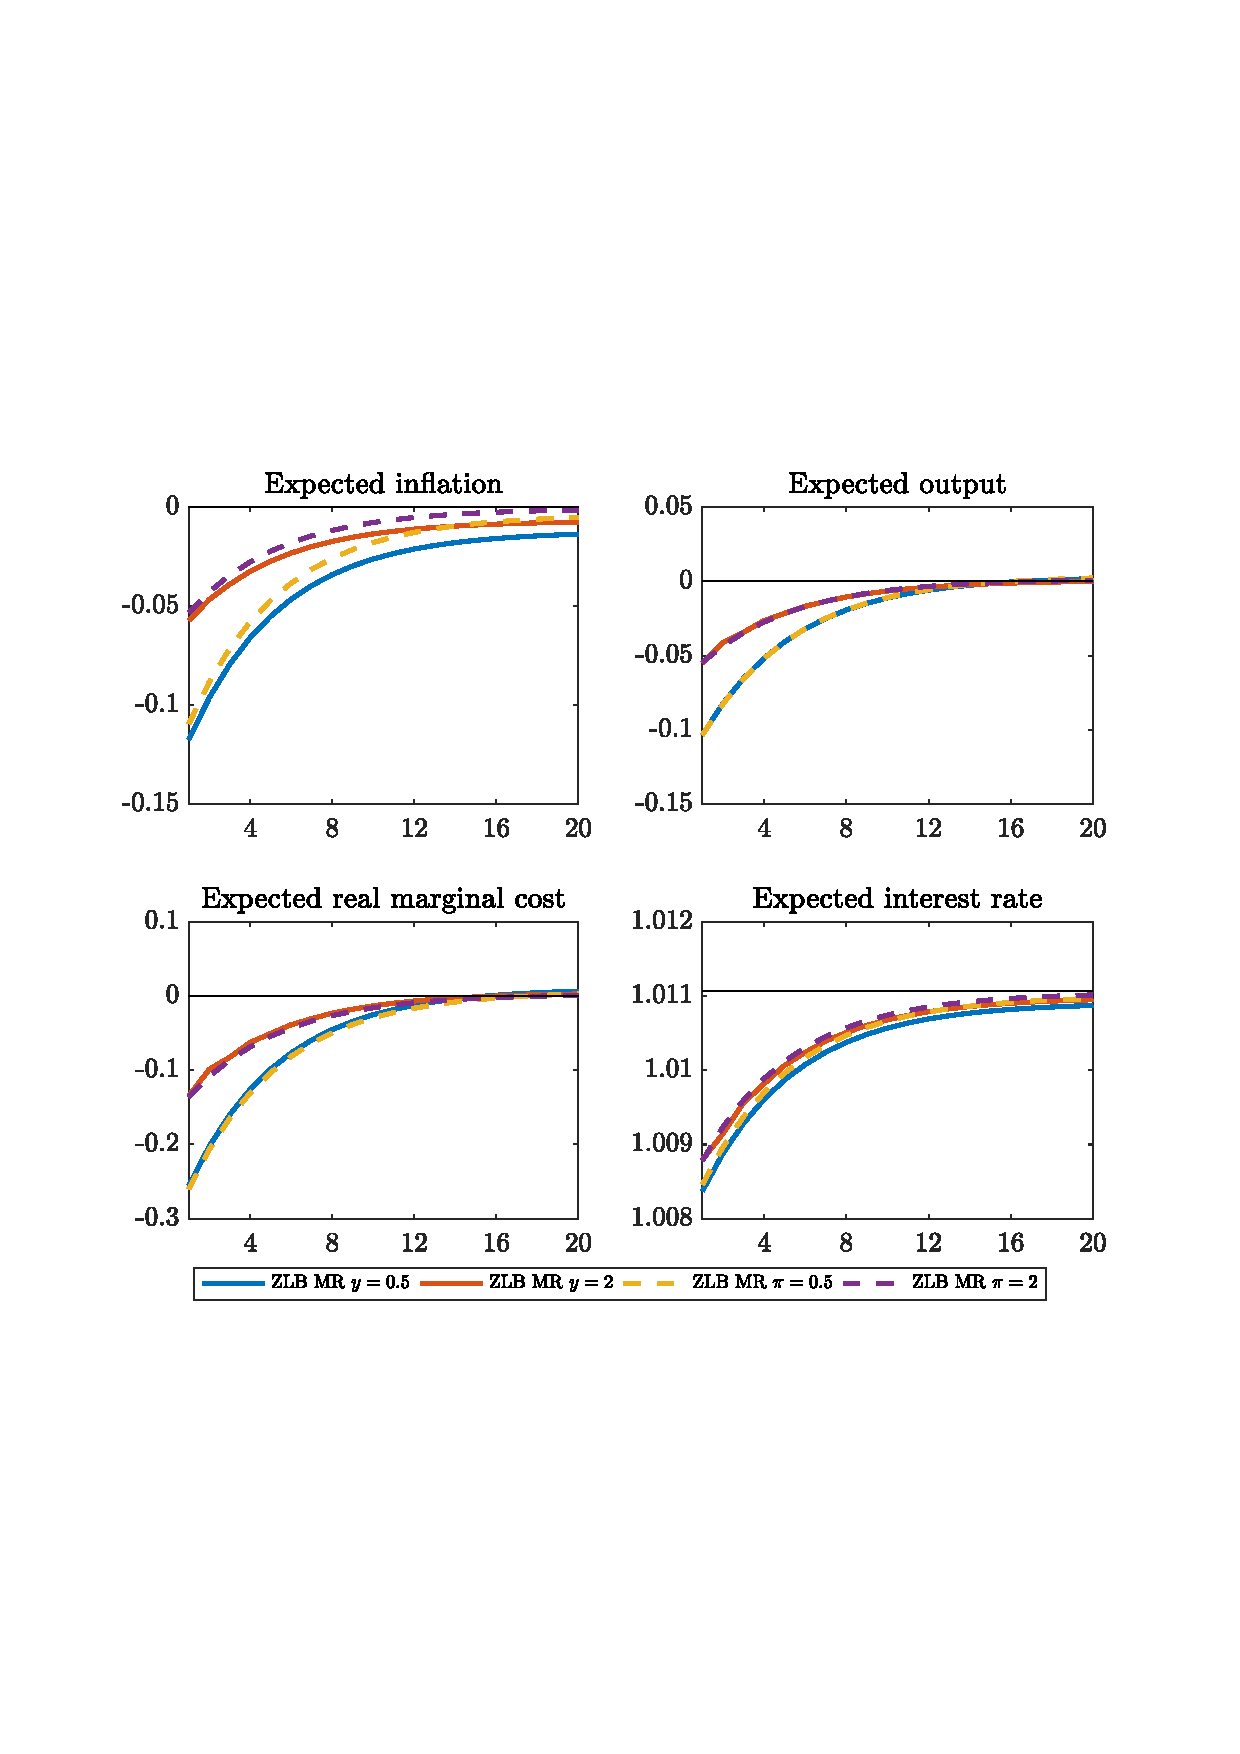
\includegraphics[scale=0.7]{irfCompDegreeExp8_pref}
%\end{figure}

\ctable[caption=Comparison between different intensities in the extended Taylor rule for expectations eight quarters ahead: impulse-responses,
	label=fig:irfCompDegreeExp8_pref,
	figure,
	notespar,
	pos=H]{c}{{\sc Notes:} Blue and red solid lines corresponds to the model when the central bank sets the interest rate using current inflation and output and also past output, where the level of importance of this last variables is of 0.5 and 2, respectively. Yellow and purple dashed lines corresponds to the model when the central bank sets the interest rate using current inflation and output and also past output, where the level of importance of this last variables is of 0.5 and 2, respectively. Expectations are computed as recursive one-step-ahead forecast over simulations. All responses to a negative demand shock, which corresponds to a one period increment in the discount factor. All responses plotted as percentage differences with respect to their steady state values, except interest rate which is plotted in gross terms.}
{
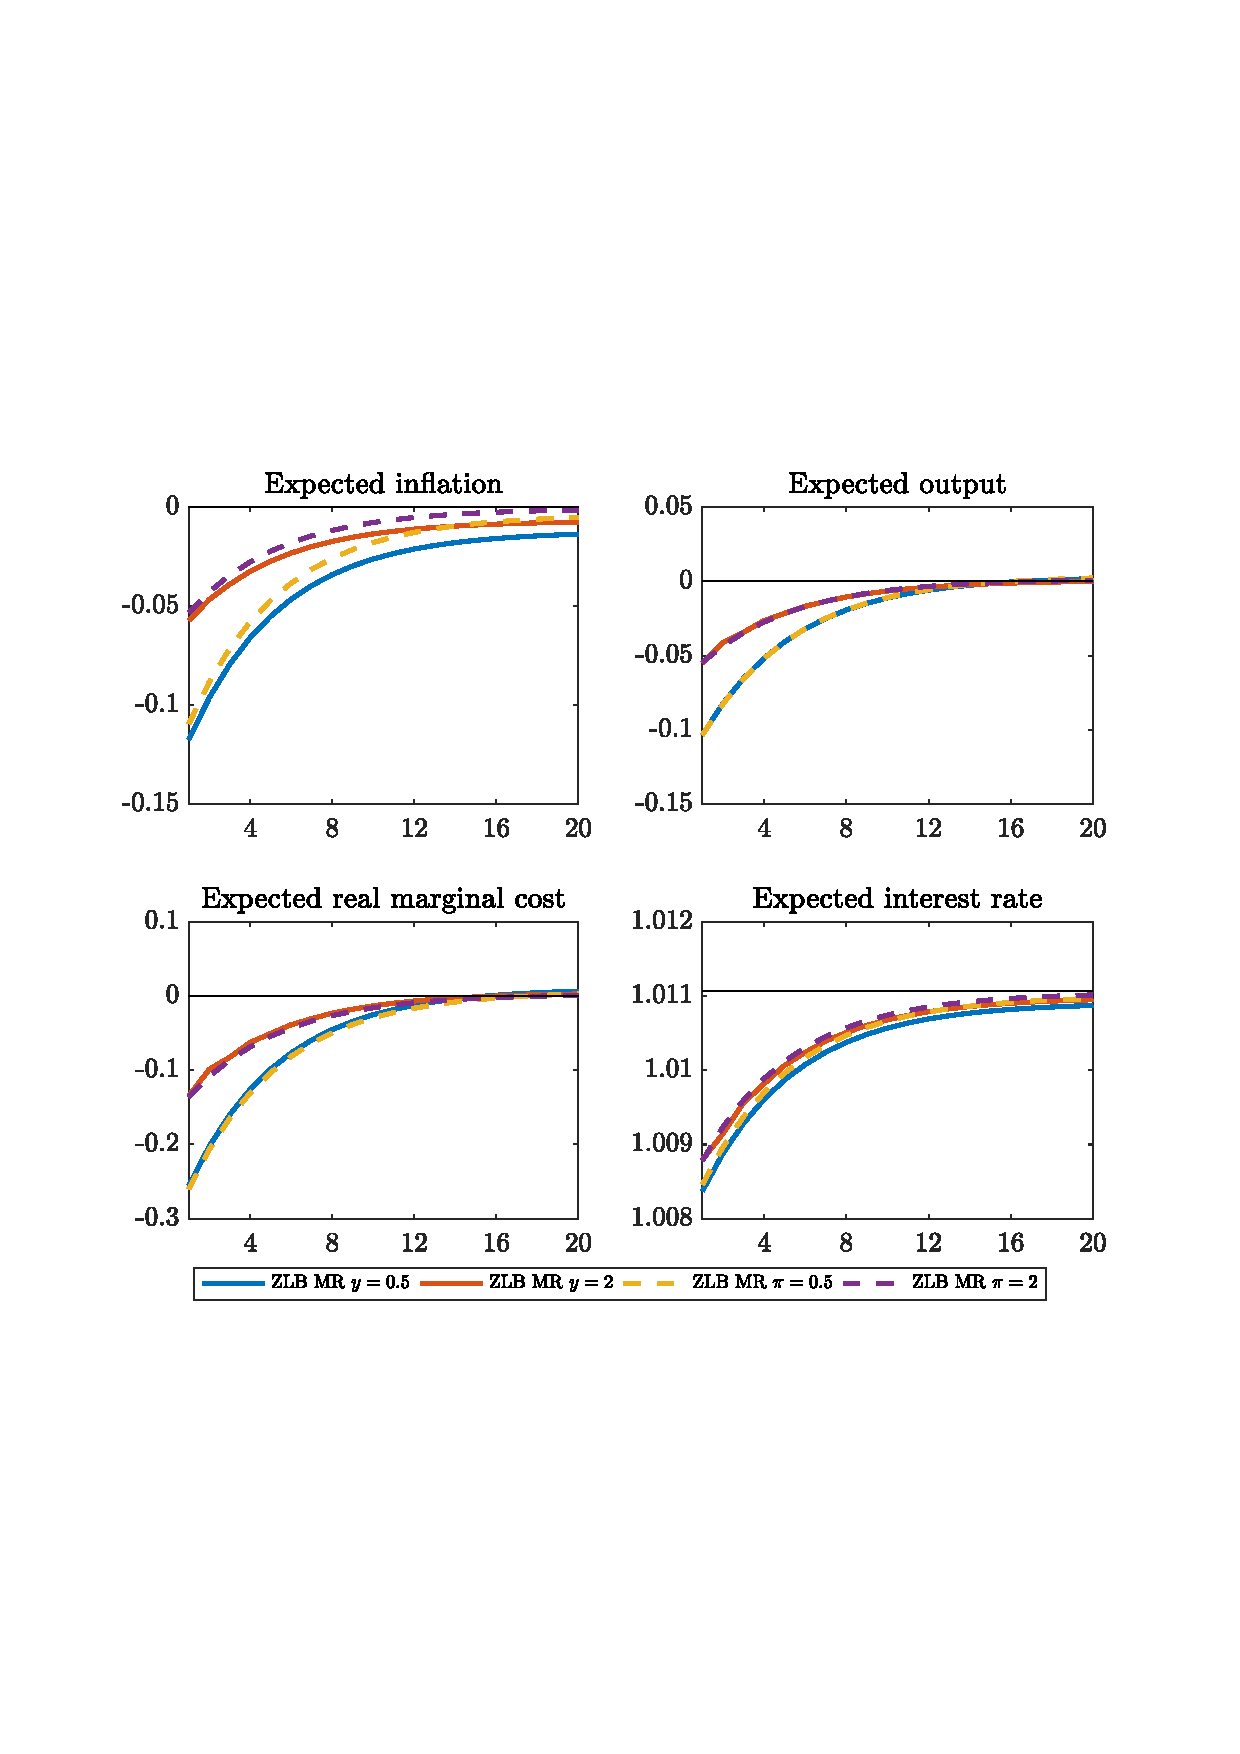
\includegraphics[scale=.6]{irfCompDegreeExp8_pref}
}

My second exercise to analyze the characteristics of the model under different Taylor rules is to compare the long-run distribution of the variables under the cases studied before. In Figure \ref{fig:distLevel}, I plot the ergodic distribution of the variables in the model. To do this, I simulate the economy for 50,000 periods and compute the relevant distributions. On each panel, the vertical line corresponds to the deterministic steady state value of the respective variable. From this exercise we can obtain two conclusions. First, in all cases variables are distributed more closely to their long-run value when the rule is more aggressive. Because the monetary authority reacts strongly to shocks, the economy comes back quickly to the long-run equilibrium, so variables present less dispersion. Also, in those cases there is less mass on the tails, which implies that extreme variations in any of these variables are less likely when the monetary authority reacts more strongly to changes in macroeconomic conditions. This last result is more remarkable in the case of real marginal costs, where extreme decreases are observed in equilibrium with the conventional rule. Second, the frequency of the zero lower bound is dramatically reduced. In the case of conventional Taylor rule we observe a frequency of 2.046\%, while in the cases with $\phi_{FG}=0.5$ and 2 we observe frequencies of 0.332 and 0.076\%, respectively. This reinforces the previous intuition that the monetary authority avoids to fall in a liquidity trap when conducting monetary policy, hence, when considers an expanded Taylor rule internalizes the consequences of the zero lower bound and use it only when necessary. It is interesting to note also that even in the case with a small degree of persistence of past output ($\phi_{FG}=0.5$) the frequency in which the economy attains the zero lower bound is significantly reduced.

%\begin{figure}[H]
%	\centering
%	\caption{Comparison between different intensities in the extended Taylor rule: long-run distributions}\label{fig:distLevel}
%	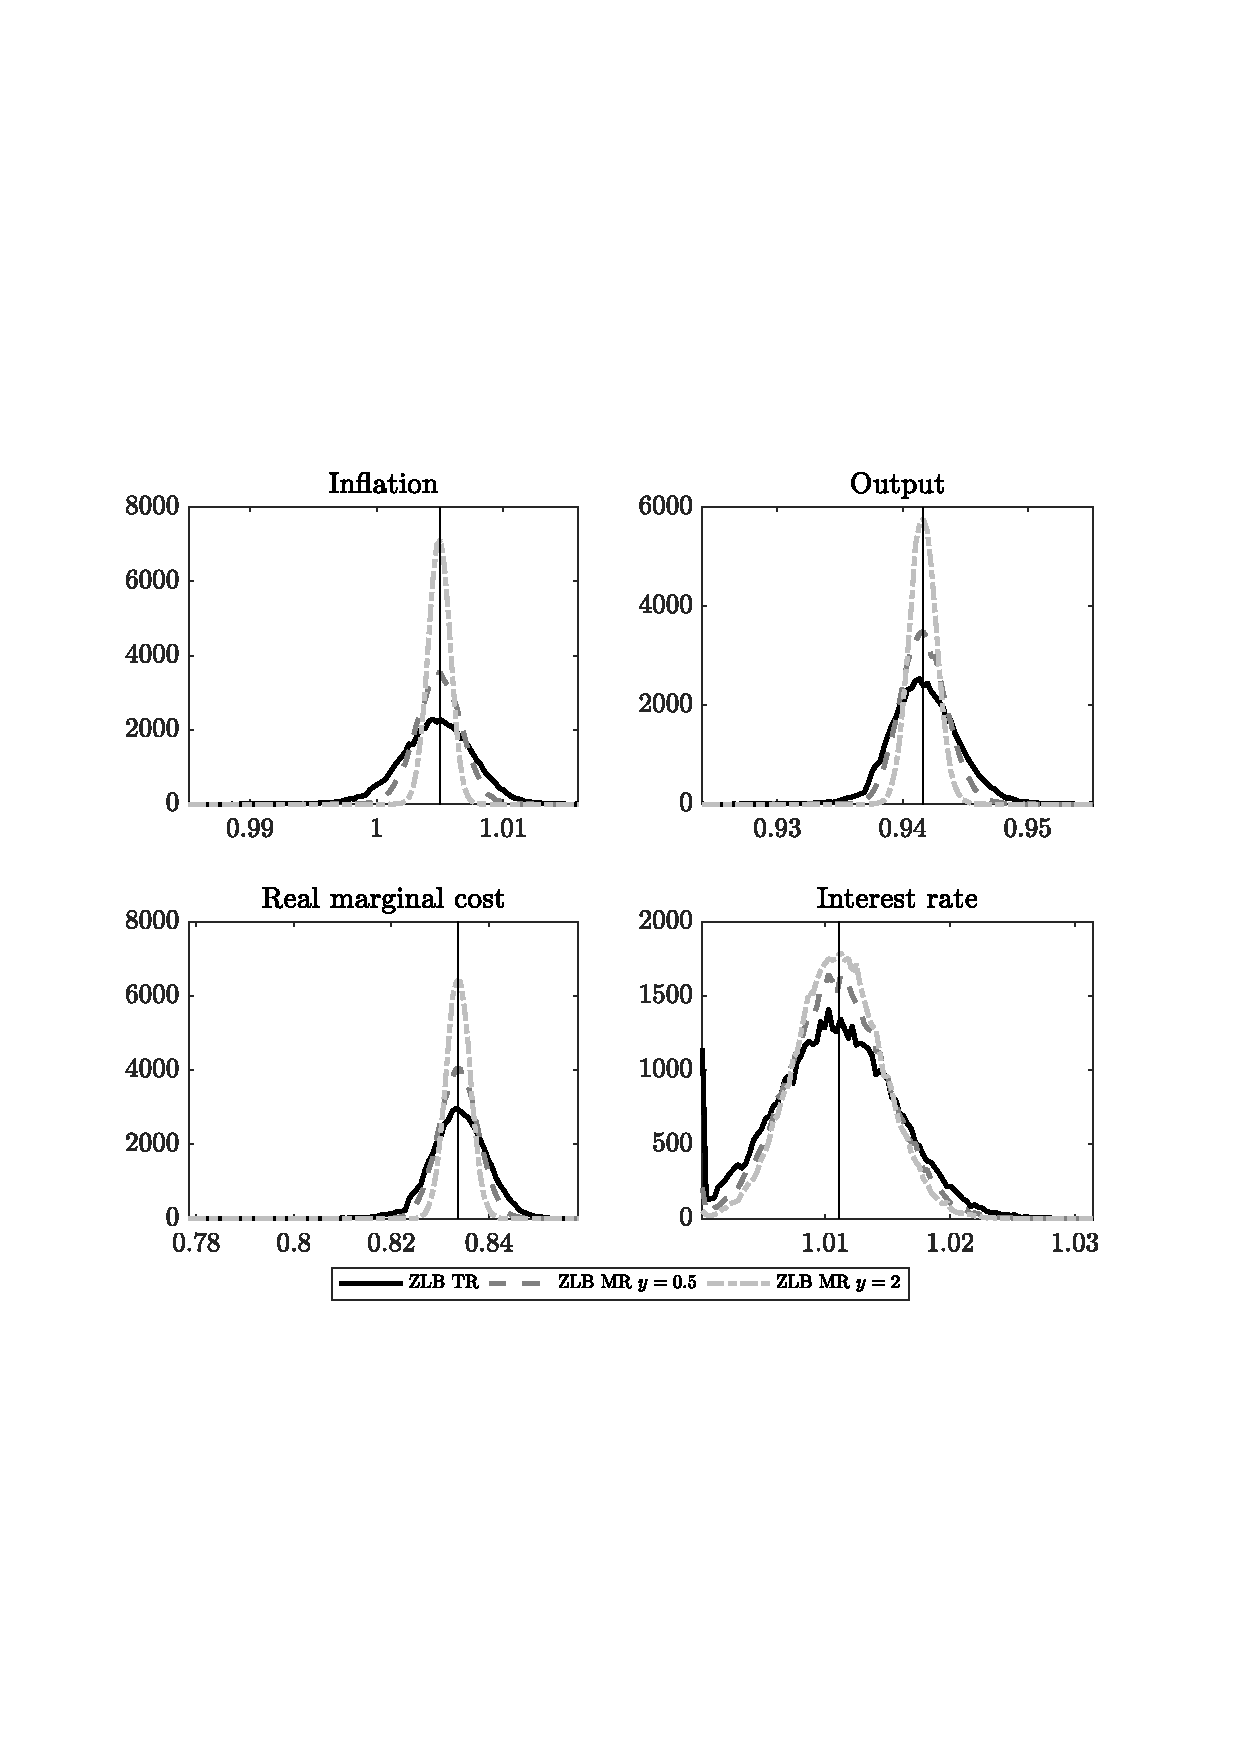
\includegraphics[scale=0.7]{distLevel}
%\end{figure}

\ctable[caption=Comparison between different intensities in the extended Taylor rule: long-run distributions,
	label=fig:distLevel,
	figure,
	notespar,
	pos=H]{c}{{\sc Notes:} All figures show the ergodic distribution of the respective variable over a simulation of 50,000 periods, considering the zero lower bound as an active constraint. Black solid line is the distribution when the Taylor rule only considers current inflation and output for the interest rate determination. Dashed darker grey line is the distribution when the Taylor rule also considers past output for the interest rate determination, with a sensitivity of 0.5. Dashed lighter grey line is the distribution when the Taylor rule also considers past output for the interest rate determination, with a sensitivity of 2. All variables are presented in gross terms. Vertical lines corresponds to the deterministic steady state of the variable.}
{
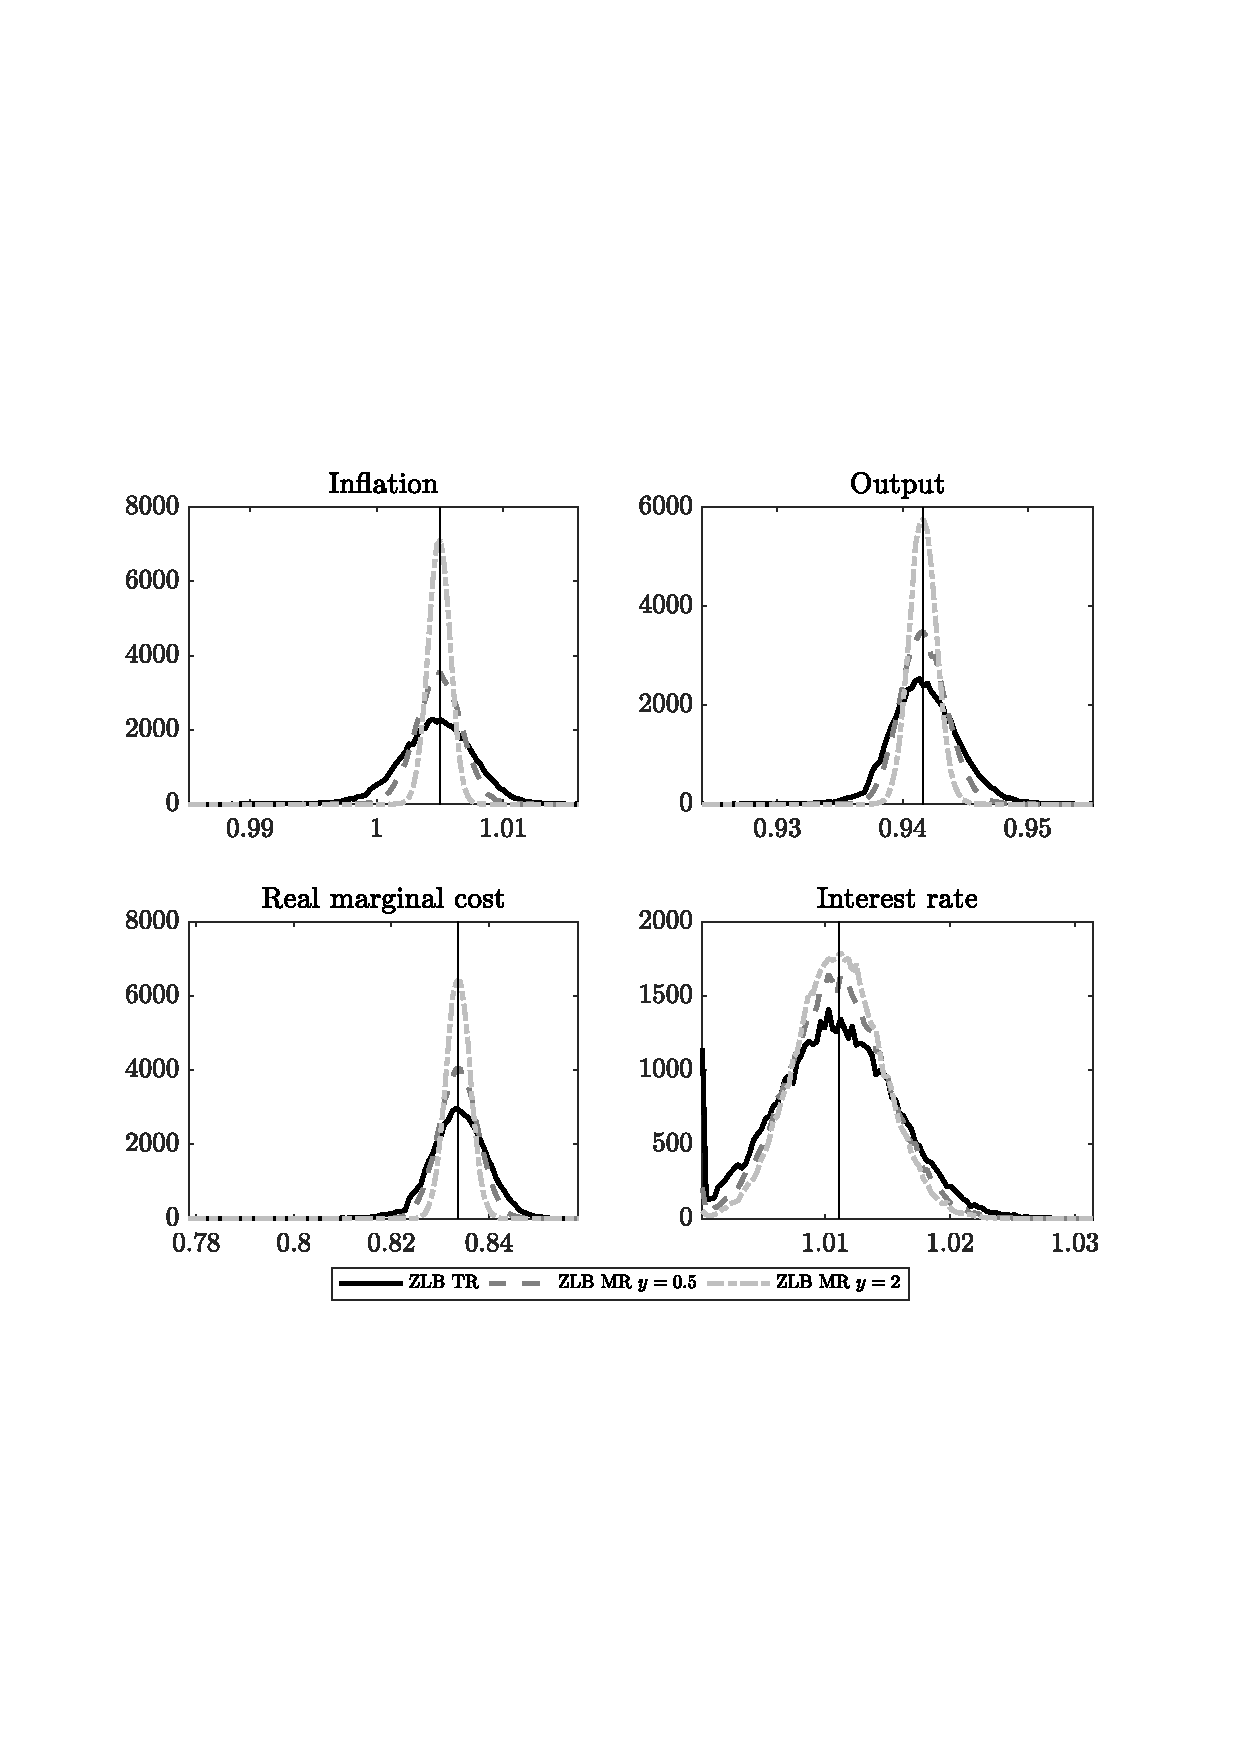
\includegraphics[scale=.6]{distLevel}
}

The last exercise to compare different rules is a welfare one. Using the simulation of the shock and the simulation of the model, I compute flow utility on each period and the corresponding discount factor which is $\prod_{i=0}^t\beta_i, \forall t=0,...,\infty$. Then, I compute the aggregate utility of the household as $\sum_{t=0}^{\infty}(\prod_{i=0}^t\beta_i)U(C_t,N_t)$. The larger the utility level, the larger is the level of welfare in the economy. In Table \ref{tab:welfare}, I present the level of welfare as a function of the intensity of past values in the expanded Taylor rule ($\phi_{FG}$), while in Figure \ref{fig:welfare}, I show the long-run distribution of utility for some selected values. In the table, the first value ($\phi_{FG}=0$) is the standard Taylor rule where only contemporaneous variables are relevant for the authority. The rest of selected values are 0.1, 0.5, 0.7, 1, 1.2, 1.5, 1.7 and 2. From this table we learn that the more intensive the monetary authority is, in terms of larger values of $\phi_{FG}$, the larger is the level of welfare of the representative household. Although modest, these increments reinforces the gains--presented along the paper--of conducting monetary policy by explicitly consider past values in its determination, specially from a long-run perspective. A second lesson comes from the figure. This shows that the tighter the monetary policy, the less likely are extreme utility losses for the household because the authority reacts quicker, taking into account the dynamic effect of its policy. With this, it can stabilize more successfully the economy and hence avoid large welfare losses. This result is relevant to understand the gains of these kinds of policies during the business cycle, not only from an stabilization perspective, but also from a social welfare one.

% Table generated by Excel2LaTeX from sheet 'Welfare'
\begin{table}[H]
  \centering
  \caption{Comparison between different intensities in the extended Taylor rule: welfare}
  \resizebox{\textwidth}{!}{ 
    \begin{tabular}{lccccccccc}
    \toprule
    $\phi_{FG}$ & 0     & 0.1   & 0.5   & 0.7   & 1     & 1.2   & 1.5   & 1.7   & 2 \\
    \midrule
    Welfare & -273.796 & -273.784 & -273.764 & -273.759 & -273.756 & -273.755 & -273.753 & -273.753 & -273.752 \\
    \bottomrule
    \end{tabular}}
  \label{tab:welfare}%
\end{table}%

%\begin{figure}[H]
%	\centering
%	\caption{Comparison between different intensities in the extended Taylor rule: welfare}\label{fig:welfare}
%	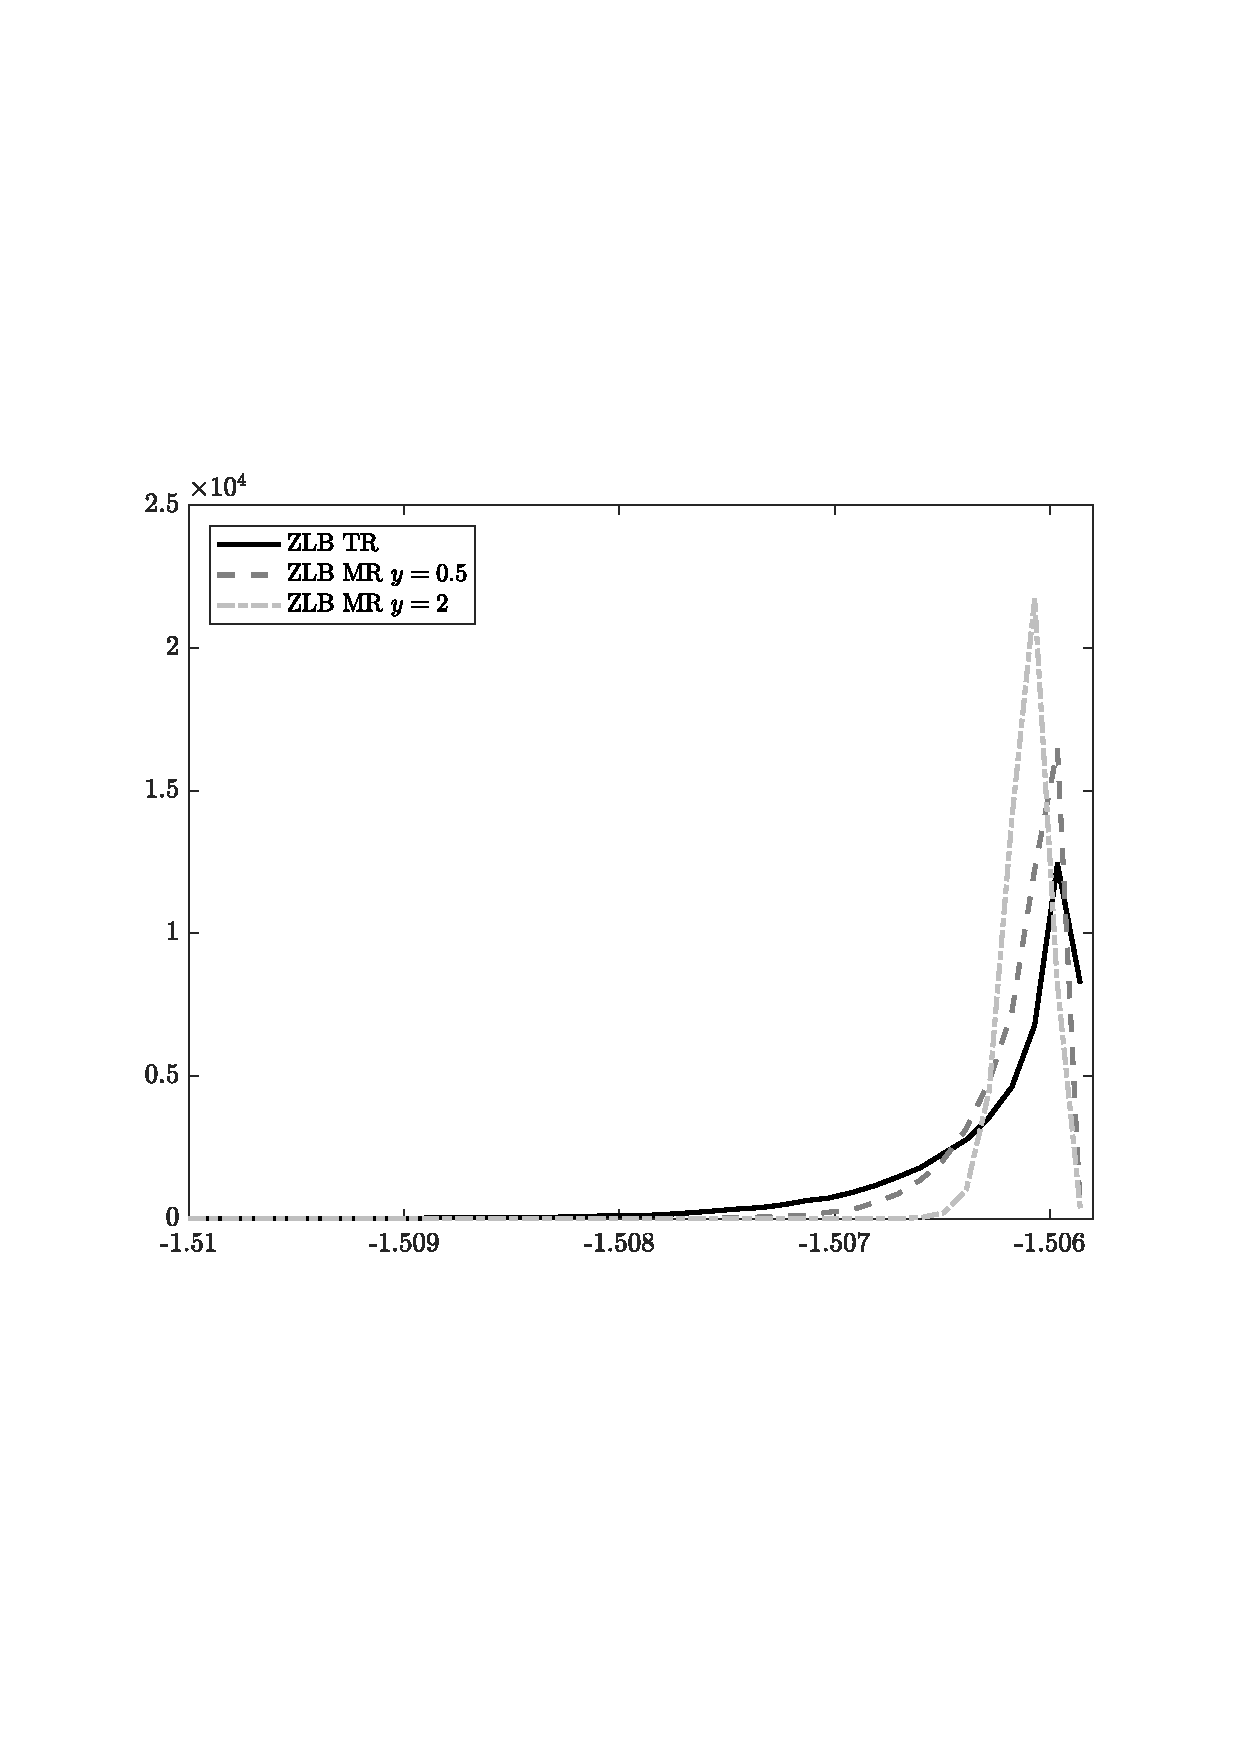
\includegraphics[scale=0.7]{welfare}
%\end{figure}

\ctable[caption=Comparison between different intensities in the extended Taylor rule: welfare,
	label=fig:welfare,
	figure,
	notespar,
	pos=H]{c}{{\sc Notes:} The figure shows the ergodic distribution of utility over a simulation of 50,000 periods. Black solid line is the distribution when the Taylor rule only considers current inflation and output for the interest rate determination. Dashed darker grey line is the distribution when the Taylor rule also considers past output for the interest rate determination, with a sensitivity of 0.5. Dashed lighter grey line is the distribution when the Taylor rule also considers past output for the interest rate determination, with a sensitivity of 2.}
{
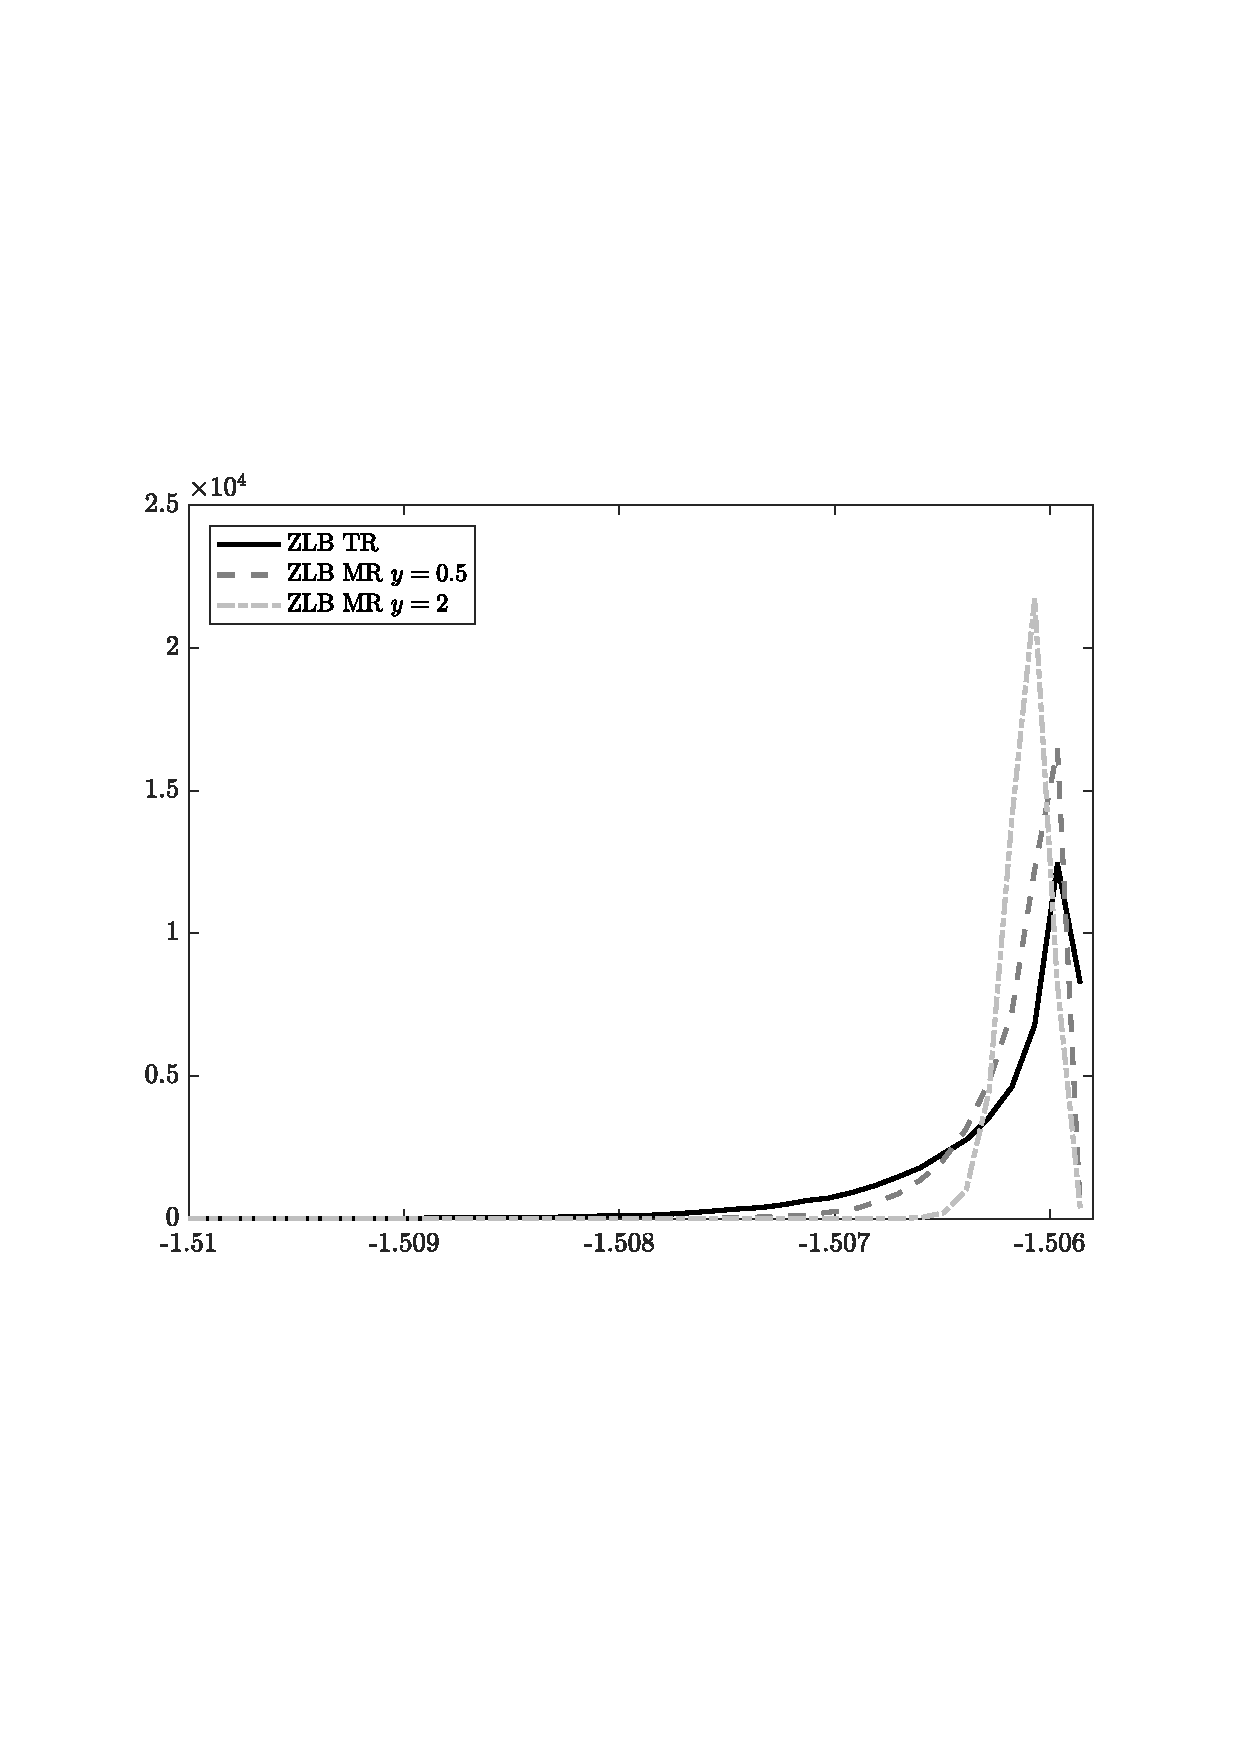
\includegraphics[scale=.6]{welfare}
}


\section{Concluding remarks}\label{sec:conclusions}

This paper analyses a New Keynesian model subject to the zero lower bound. Simulating the model when the economy responds to a large demand shock, of the form of an increase in the discount factor, I compare  the responses of variables in the model when the zero lower bound is not present, with the situation when the constrain is active. I found that when the constraint is taken into account, the central bank is less capable to react because the floor in its policy instrument is a binding constraint. In particular, after the shock, the interest rate stays at the zero lower bound for around four periods, which generates large drops on inflation, output and real marginal costs. This is a standard result in monetary economics that has just been verified in this paper. I also analyze the responses of expectations four and eight periods ahead, finding that these expectations react less in the long-run. After this, I evaluate an alternative to the standard Taylor rule typically used by the central banks, that I call modified Taylor rule or pseudo forward guidance policy. This includes a past macroeconomic variable, like output or inflation, in the standard Taylor rule, so the authority takes into account both past and current macroeconomic conditions in order to set the interest rate. I evaluate different variations in the policy, like using inflation or output and how sensitive is the authority to past variables. My results show that including any of these past variables generate gains with respect to the case without this forward guidance policy. In particular, including past inflation or output generates the same benefits, which are: (a) smaller decreases on impact in all macroeconomic variables (inflation, output and real marginal cost); (b) the zero lower bound is attained only in one period, which implies that the monetary authority uses the possibility to reach the zero lower bound in order to diminish the effects of the shock and not as a consequence of not being able to leave it before; (c) monetary policy is able to modify expectations in an horizon of at least two years in a decreasing way, which is consistent with the empirical patterns observed from the Great Recession onwards, and (d) when using the modified policy the authority is able to reduce the probability of reaching extreme outcomes in the economy, like big and large recessions, which is translated in welfare gains both in the long-run and through the business cycle. All these outcomes depend on the sensitivity of the modified Taylor rule to past level of inflation or output, but some gains are observed even in the case of a moderate response of 0.5 to deviations in past variables. All this elements are relevant for the conduct of monetary policy because reflects alternative ways of set the instruments available to the authority in order to fight an economic crisis and sustain welfare during the process.

In future research, I intend to expand the analysis presente here. In concrete, it would be interesting to analyze the model when other shocks are taken into account, like technology shocks or cost-push shocks, which are standard in the monetary literature. Also, it is important to understand the properties when the central bank selects different targets for inflation and interest rate. In this paper I have considered a positive target for both inflation and interest rate, so it should be relevant to study the consistency of my results under different targets for the authority. Finally, other interesting extensions are the relevance of fiscal policy and its joint effect with monetary policy and my modified Taylor rule, and how other unconventional policies, like quantitative easing, play a role in combination with the pseudo forward guidance.

%%GATHER{tbib.bib}
\bibliographystyle{agsm}
\bibliography{tbib}

\newpage\appendix

\section{Derivation of the model}\label{app:derivation}

In this section, I characterize the model presented in section \ref{sec:model}. In particular, I derive the optimality conditions of households and firms.

\subsection{Households}

The representative infinite-lived household wants to maximize the present value of consumption:

\begin{align*}
\mathbb{E}_t\sum_{t=0}^{\infty}\left(\prod_{j=0}^t\beta_j\right)U(C_t,N_t)
\end{align*}

where $\beta_j$ is the discount factor in period $j$, which evolves stochastically following an AR(1) process, $N_t$ is the labor offered by the household and $C_t$ is a consumption index defined as:

\begin{align*}
C_t\equiv\left(\int_0^1C_t(i)^{\frac{\epsilon-1}{\epsilon}}di\right)^{\frac{\epsilon}{\epsilon-1}}
\end{align*}

where $i$ is the index of varieties of consumption. 

The period budget constraint is:

\begin{align*}
\int_0^1P_t(i)C_t(i)di+Q_tB_t\leq B_{t-1}+W_tN_t+T_t
\end{align*}

The decision of consumption expenditures among the different goods could be summarized in the set of demand equations:

\begin{align*}
C_t(i)=\left(\frac{P_t(i)}{P_t}\right)^{-\epsilon}C_t
\end{align*}

where $P_t\equiv\left(\int_0^1P_t(i)^{1-\epsilon}di\right)^{\frac{1}{1-\epsilon}}$ is an aggregate price index.\footnote{This demands are obtained from the solution of the expenditure minimization problem, subject to the total expenditure. More formally, the problem is:

\begin{align*}
\min \left(\int_0^1C_t(i)^{\frac{\epsilon-1}{\epsilon}}di\right)^{\frac{\epsilon}{\epsilon-1}}
\intertext{subject to}
\int_0^1P_t(i)C_t(i)di\equiv Z_t
\end{align*}

where $Z_t$ is a given level of expenditure.} Conditional in this optimization, we can re-write the budget constraint as:

\begin{align*}
P_tC_t+Q_tB_t\leq B_{t-1}+W_tN_t+T_t
\end{align*}

Assuming a CES utility function like:

\begin{align*}
U(C_t,N_t)=\frac{C_t^{1-\sigma}}{1-\sigma}-\frac{N_t^{1+\varphi}}{1+\varphi}
\end{align*}

the first order conditions are:

\begin{align*}
C_t^{\sigma}N_t^{\varphi}&=\frac{W_t}{P_t}\\
1&=R_t\mathbb{E}_t\left\{\beta_{t+1}\left(\frac{C_t}{C_{t+1}}\right)^{\sigma}\frac{1}{\Pi_{t+1}}\right\}
\end{align*}

In this paper I am interested in studying the effect of demand shocks of the form of variations in the discount factor. Given this, the discount factor is time-varying and must be included into the expected value.

\subsection{Firms}

\subsubsection{Production function}

Given that we have a continuum of varieties of consumption, we also have a continuum of firms producing those. We assume the following technology:

\begin{align*}
Y_t(i)=N_t(i)
\end{align*}

Given this production function, we know that the total cost of the firm ($CT_t$) is:

\begin{align*}
CT_t=W_tY_t
\end{align*}

So the marginal cost is just $W_t$, which in real terms (real marginal cost, $RMC_t$) is $RMC_t=W_t/P_t$.

\subsubsection{Price dynamics}

In this section I change the assumption of Calvo pricing and replace it with Rotemberg pricing. Following \cite{AscariEtAl2012} and \cite{Rotemberg1982}, I assume the following adjustment cost function for prices:

\begin{align*}
\frac{\zeta}{2}\left(\frac{P_t(i)}{P_{t-1}(i)}-1\right)^2Y_t
\end{align*}

Then, the problem of each firm is:

\begin{align*}
&\max_{P_t(i)} \mathbb{E}_t \sum_{k=0}^{\infty}Q_{t,t+k}\left[\left(\frac{P_{t+k}(i)}{P_{t+k}} - RMC_{t+k} \right)Y_{t+k}(i) - \frac{\zeta}{2}\left(\frac{P_t(i)}{P_{t-1}(i)}-1\right)^2Y_t\right]\\
&\text{st} \quad Y_t(i)=\left(\frac{P_t(i)}{P_t}\right)^{-\epsilon}Y_t
\end{align*}

where $Q_{t,t+k}$ is the discount factor of each firm in period $t$ for profits in period $t+k$. Replacing the restriction into the objective function we have:

\begin{align*}
&\max_{P_t(i)} \mathbb{E}_t \sum_{k=0}^{\infty}Q_{t,t+k}\left[\left(\frac{P_{t+k}(i)}{P_{t+k}} - RMC_{t+k} \right)\left(\frac{P_{t+k}(i)}{P_{t+k}}\right)^{-\epsilon}Y_{t+k} - \frac{\zeta}{2}\left(\frac{P_t(i)}{P_{t-1}(i)}-1\right)^2Y_t\right]\\
&\max_{P_t(i)} \mathbb{E}_t \sum_{k=0}^{\infty}Q_{t,t+k}\left[\left(\left(\frac{P_{t+k}(i)}{P_{t+k}}\right)^{1-\epsilon} - RMC_{t+k}\left(\frac{P_{t+k}(i)}{P_{t+k}}\right)^{-\epsilon} \right)Y_{t+k} - \frac{\zeta}{2}\left(\frac{P_t(i)}{P_{t-1}(i)}-1\right)^2Y_t\right]
\end{align*}

The first order condition is:

\begin{align*}
&\left[(1-\epsilon)\left(\frac{P_{t}(i)}{P_{t}}\right)^{-\epsilon}\left(\frac{1}{P_t}\right)+\epsilon RMC_t \left(\frac{P_{t}(i)}{P_{t}}\right)^{-\epsilon-1}\left(\frac{1}{P_t}\right)\right]Y_t-\zeta\left(\frac{P_t(i)}{P_{t-1}(i)}-1\right)\left(\frac{Y_t}{P_{t-1}}\right)\\
&+\mathbb{E}_t\left\{Q_{t,t+1}\left[\zeta\left(\frac{P_{t+1}}{P_t}-1\right)\left(\frac{P_{t+1}}{P_t^2}\right)Y_{t+1}\right]\right\}=0
\end{align*}

Imposing a symmetric equilibrium condition, $P_t(i)=P_t$, we have:

\begin{align*}
[(1-\epsilon)+\epsilon RMC_t]\left(\frac{Y_t}{P_t}\right)-\zeta\left(\frac{P_t(i)}{P_{t-1}(i)}-1\right)\left(\frac{Y_t}{P_{t-1}}\right)\\
+\mathbb{E}_t\left\{Q_{t,t+1}\left[\zeta\left(\frac{P_{t+1}}{P_t}-1\right)\left(\frac{P_{t+1}}{P_t^2}\right)Y_{t+1}\right]\right\}=0
\end{align*}

Multiplying the previous expression by $P_t/Y_t$ and defining inflation as $\Pi=P_t/P_{t-1}$:

\begin{align*}
(1-\epsilon)+\epsilon RMC_t-\zeta(\Pi_t-1)\Pi_t=-\mathbb{E}_t\left\{Q_{t,t+1}\left[\zeta(\Pi_{t+1}-1)\Pi_{t+1}\frac{Y_{t+1}}{Y_t}\right]\right\}
\end{align*}

where the stochastic discount factor in period $t+1$ is $\beta_{t+1}(C_t/C_{t+1})^{\sigma}$. Finally we have:

\begin{align*}
(1-\epsilon)+\epsilon RMC_t-\zeta(\Pi_t-1)\Pi_t=-\mathbb{E}_t\left\{\beta_{t+1}\left(\frac{C_t}{C_{t+1}}\right)^{\sigma}\left[\zeta(\Pi_{t+1}-1)\Pi_{t+1}\frac{Y_{t+1}}{Y_t}\right]\right\}
\end{align*}

\section{Accuracy tests}\label{app:accuracy}
	
In this section, I present the accuracy tests described in the main text. As was mentioned before, I compute residuals in the Euler equation and residuals in the New Keynesian Phillips curve using a larger grid (100 points). Also, I compute the relative approximation error in terms of consumption. All the statistics are presented on average and also as the maximum absolute value. Results are presented in Table \ref{tab:app_error}. On each panel I show a different version of the modified Taylor rule, where the first one is the case where no past variables are considered in the policy rule.

% Table generated by Excel2LaTeX from sheet 'Residual errors 2'
\begin{table}[H]
  \centering
  \caption{Approximation errors of the solutions ($\times 100$)}
  \begin{threeparttable}
        \begin{tabular}{lccccrlccc}
    \toprule
          & \multicolumn{4}{c}{Taylor rule with past output} &       & \multicolumn{4}{c}{Taylor rule with past inflation} \\
    \cline{2-10}
          & (1)   & (2)   & (3)   & (4)   &       & \multicolumn{1}{c}{(1)} & (2)   & (3)   & (4) \\
    \midrule      
          & \multicolumn{9}{c}{$\phi_{FG}=0$} \\
	\midrule          
    No ZLB & -0.0006 & 0.0460 & -0.0002 & 0.0017 &       & \multicolumn{1}{c}{-0.0006} & 0.0460 & -0.0002 & 0.0017 \\
    ZLB   & 0.0180 & 0.1804 & -0.0030 & 0.0450 &       & \multicolumn{1}{c}{0.0180} & 0.1804 & -0.0030 & 0.0450 \\
          &       &       &       &       &       &       &       &       &  \\
	\midrule          
          & \multicolumn{9}{c}{$\phi_{FG}=0.5$} \\
	\midrule          
    No ZLB & 0.0010 & 0.0341 & -0.0002 & 0.0015 &       & \multicolumn{1}{c}{-0.0006} & 0.0353 & -0.0001 & 0.0015 \\
    ZLB   & 0.0121 & 0.3116 & -0.0019 & 0.1554 &       & \multicolumn{1}{c}{0.0118} & 0.2833 & -0.0020 & 0.1413 \\
          &       &       &       &       &       &       &       &       &  \\
	\midrule          
          & \multicolumn{9}{c}{$\phi_{FG}=1$} \\
	\midrule          
    No ZLB & 0.0004 & 0.0403 & -0.0001 & 0.0014 &       & \multicolumn{1}{c}{-0.0017} & 0.0489 & 0.0000 & 0.0017 \\
    ZLB   & 0.0082 & 0.7838 & 0.0000 & 0.3896 &       & \multicolumn{1}{c}{0.0049} & 0.7419 & 0.0005 & 0.3689 \\
          &       &       &       &       &       &       &       &       &  \\
	\midrule          
          & \multicolumn{9}{c}{$\phi_{FG}=2$} \\
    \midrule      
    No ZLB & -0.0016 & 0.0585 & -0.0001 & 0.0014 &       & \multicolumn{1}{c}{-0.0061} & 0.1071 & 0.0002 & 0.0029 \\
    ZLB   & -0.0076 & 1.6002 & 0.0128 & 0.7844 &       & \multicolumn{1}{c}{-0.0091} & 1.5140 & 0.0112 & 0.7485 \\
    \bottomrule
    \end{tabular}%
    \begin{tablenotes}
    	{\footnotesize {\sc Notes:} Column (1) shows average residual from the model. Column (2) shows the maximum absolute residual from the model. Column (3) shows the average relative consumption error. Column (4) shows the maximum absolute consumption error. Each panel corresponds to a different version of the modified Taylor rule. All figures have been multiplied by 100.}
    \end{tablenotes}
	\end{threeparttable}	
  \label{tab:app_error}%
\end{table}%
	
\end{document}